%********************************************************** 
% Version 0.1 Junying Chen, 1/8/2012
% Version 0.2 Cheng Liu, 20/4/2015
%*********************************************************


\documentclass[12pt,a4paper]{report}
\usepackage{setspace} % Set line spacing package
\doublespacing
\usepackage[binary-units]{siunitx}
\usepackage{mathptmx} % Times Roman typeface
\usepackage[latin1]{inputenc}
\usepackage{amsmath}
\usepackage{amsfonts}
\usepackage{amssymb}
\usepackage{float}
\usepackage{graphicx}
\graphicspath{{./figures/}}
\usepackage[small]{caption} % Small font size of figure caption
\usepackage{caption}
\usepackage{subfigure}
\usepackage{enumerate}
\usepackage{bm}

% algorithm package
\usepackage{algorithm}
\usepackage{algorithmic}
\usepackage[algo2e]{algorithm2e}
\renewcommand{\algorithmcfname}{ALGORITHM}

% citation package
\usepackage[numbers, sort&compress]{natbib}

% hyperlink
\usepackage[linktoc=all, bookmarks=true]{hyperref}

%% Additional packages
\usepackage{times,amsmath,epsfig}
\usepackage{verbatim}
\usepackage{array}
\usepackage{multirow}

%\usepackage[margin=1.5cm]{geometry}  % the easy way to set page margins
\usepackage[top=25mm, bottom=25mm, left=35mm, right=35mm]{geometry}

\usepackage{url} % Add online resources in references

% references commands
\newcommand{\eqnref}[1]{(\ref{#1})}
\newcommand{\figref}[1]{Figure~\ref{#1}}
\newcommand{\secref}[1]{Section~\ref{#1}}
\newcommand{\chapref}[1]{Chapter~\ref{#1}}
\newcommand{\tabref}[1]{Table~\ref{#1}}
\newcommand{\algref}[1]{Algorithm~\ref{#1}}
\newcommand{\code}[1]{\texttt{#1}}
\newcommand{\tabincell}[2]{\begin{tabular}{@{}#1@{}}#2\end{tabular}}

%\def\PDFFIG[#1]#2#3#4{  %[#parameter]#image_name#caption#label
%\begin{figure}[H]
%\centering
%\includegraphics[#1]{#2}
%\caption{#3}
%\label{#4}
%\end{figure}
%}

\begin{document}
% Front Page with Abstract

\begin{center}
\small Abstract of thesis entitled

\LARGE "QuickDough: A Rapid FPGA Loop Accelerator Design Framework Using Soft Coarse-Grained
Reconfigurable Array Overlay"

\vspace{5mm}
\small Submitted by 

\large \textbf{Cheng LIU}

\vspace{5mm}
for the degree of Doctor of Philosophy \\
at The University of Hong Kong \\
in December 2015 \\

\vspace{5mm}
\end{center}
The QuickDough design framework is presented as a way to address productivity issues of developing
high-performance FPGA accelerators. QuickDough utilizes a soft coarse-grained reconfigurable array
(SCGRA) as an overlay on top of off-the-shelf FPGAs for rapid accelerator developments.
Instead of compiling high-level applications directly to HDL circuits, the compilation step is
reduced to a simpler operation scheduling task targeting the SCGRA overlay, significantly reducing
compilation time and increasing possible numbers of debug-cycle-per-day as a result.
The softness of the SCGRA allows highly customized application-specific design while the regular
structure of the SCGRA makes the customization much easier. When compared to the
execution on a general purposed processor, the accelerators generated using QuickDough achieves up
to 9X performance speedup.


\begin{center}
\rule{60mm}{0.4pt} \\
\emph{An abstract of exactly 436 words.}
\end{center}

\pagebreak

\input{cover}
\hfill

%\begin{figure}
%\centering
%\includegraphics[width=0.15\columnwidth]{HKUshield}
%\end{figure}

%%============================================================

\newpage
\pagenumbering{Roman}
\section*{\centering{Declaration}}

% Thesis statement of originality -------------------------------------

% Depending on the regulations of your faculty you may need a declaration like the one below. This specific one is from the medical faculty of the university of Dresden.



I hereby declare that this thesis represents my own work, except where due acknowledgment is made, and that it has not been previously included in a thesis, dissertation or report submitted to this university or to any other institution for a degree diploma or other qualifications.

\vspace{20mm}

\begin{flushright}
\textit{Signature: }\rule{5cm}{0.5pt}\\
Cheng Liu \qquad\qquad\qquad\qquad
\end{flushright}




% ----------------------------------------------------------------------

\hfill

%%============================================================
\newpage
\section*{\centering{Acknowledgement}}
I would like to express profound gratitude to my supervisor in Department of Electrical and Electronic Engineering from The University of Hong Kong, Dr. Hayden Kwok-Hay So. Thank you for giving me numerous suggestions, encouragement and support for this QuickDough research project. Without his guide, this thesis would not be possible. I really appreciate the way you solve problems and the rule you do research. I believe these will be beneficial to the rest of my life.

I would like to thank Dr. Ngai Wong. Although he is not doing research exactly on reconfigurable computing, he gave me a lot of great general suggestions on doing research in the first semester of my PhD study when everything was completely new for me. He also spent quite a lot of efforts pushing me to the right track of doing research and encouraged me when I was confused. 


I want to thank the lab mates including Colin, Candice, Mingo, Ho-Cheung and Sam for all the help on my research. Most importantly, I would like to thank you for showing me the various woderful food hiding in Hong Kong. I would like to thank Sharat who gave me a lot of suggestions on the QuickDough project as well. At the same time, I want to thank the buddies including Xiachun Chen, Fang Liu, Ya Wei, Xiaoxu Shi, Big Brother Qun, Prof.Fang, Ruihua Ye and so on for climbing the hills in HK when I was extremely discouraging on my research. It was really helpful to release the stress and resume courage on my PhD study.

Finally, I would thank my family for all the support and understanding on my study in HKU. 

\hfill

%%============================================================

%\newpage
%\section*{\centering{List of Publication}}
%\input{publist}
%\hfill
%
%%============================================================
\tableofcontents
\cleardoublepage

\listoffigures	% print list of figures
\listoftables  % print list of tables

%%============================================================
\chapter{Introduction} \label{chapter:intro} 
Recent years have witnessed a tremendous growth in the use of accelerators in computer systems to improve the systems' performance and energy efficiency \cite{kim2014compression, majumder2014hardware, iouliia2004reconfigurable, souradip2010hardware, putnam2014reconfigurable}. Among these accelerators, GPUs and Xeon Phi accelerators have stood out as two of the most popular choices in spite of their relatively short history as accelerators--5 of the top 10 systems on the top500 list take advantage of them \cite{top500}. On the other hand, despite the long and successful track record of FPGA accelerators with promising performance speedup and energy efficiency \cite{iouliia2004reconfigurable, souradip2010hardware, asano2009performance, che2008accelerating, thomas2009comparison}, the use of FPGA accelerators in main-stream systems remains limited and has yet to receive widespread adoption beyond highly skilled hardware engineers \cite{cong2011high}. When compared to the wide adoption of GPUs and Xeon Phi accelerators, it is believed that the much lower design productivity in developing FPGA applications, which is generally caused by both the lengthy FPGA compilation and notorious inaccessibility to software programmers, has become one of the major obstacles that hinder the software developers using FPGAs as compute accelerators. 

When considering the classical hardware description language (HDL) based FPGA accelerator development flow, a number of aspects lead to the FPGA design productivity challenge. First of all, the FPGA design process using HDL is fundamentally different from that of software development and requires the low-level circuit design techniques which most of the software designers are unfamiliar with. In addition, the relatively low abstraction level of hardware description languages also limits the efficiency of the application development and thus the designers' productivity eventually \cite{cong2011high}. Secondly, instead of spending seconds to compile and debug a quick-and-dirty proof-of-concept design, software programmers soon find that implementing even the smallest FPGA design consumes at least tens of minutes. As the size of their designs increases, the run-time of the implementation tools quickly goes up to hours or even days, greatly limiting the number of possible debug-edit-compile cycles per day \cite{lavin2010using, lavin2011HMFlow, korf2011automatic, yue2015rapid}. Beyond that, software designers are often put off by the large amount of design optimization options involved in both the design tools and the hardware designs. Moreover, the initial hardware design can rarely meet the requirements and the design optimization is critical to achieve the anticipated performance and energy-efficiency \cite{schafer2012machine, zhong2014design, holzer2007design, schafer2012divide, liu2013learning, kurek2014automating}. 

Although both the industry and academia have made significant progress in increasing the productivity of the FPGA designers by improving the EDA tools for shorter run time \cite{VivadoHLS, mulpuri2001runtime, moctar2014parallel, goeders2011deterministic} and providing a large amount of IPs for design reuse \cite{xilinx-pc, altera-pc}, the typical FPGA compilation remains two orders of magnitudes slower than software compilation and the FPGA accelerator design remains a discipline mostly carried out by highly trained specialists. The full potential of FPGAs to the software programmers hasn't been fully unleashed and there is still a long way to drive towards software programmable FPGA allowing high-productivity FPGA development \cite{fsp2014, fsp2015}.

\section{High-level Synthesis}
To bridge the design productivity gap between software and hardware development, many people have turned to the use of high-level synthesis (HLS) techniques in the past decades \cite{cong2011high}. \figref{fig:hls-compilation} presents both the FPGA design flow using conventional hardware description language (HDL) and HLS. It is clearly that the HDL based FPGA design flow takes HDL as the design entry and thus requires the users to be experienced on low-level circuit design to develop a register-transfer level (RTL) FPGA accelerator for an application. By raising the abstraction level of the physical hardware, HLS based design flow allows designers to develop hardware using familiar high-level, software-like description languages such as C, C++, C-like languages, Matlab and Python \cite{handel-c, ROCCC, VivadoHLS, OpenCL, matlab, myhdl}. The low-level hardware implementations are then left to the conventional design tools to synthesize and optimize. With decades of efforts, some early results in HLS have already found their ways into FPGA vendors' commercial tools in recent years \cite{OpenCL, VivadoHLS, handel-c, zhang2008autopilot, chen2005xpilot}. 

\begin{figure}
\centering
\includegraphics[width=0.65\linewidth]{hls-compilation}
\caption{FPGA Design Flow Using Conventional HDL and HLS.}
\label{fig:hls-compilation}
\end{figure}

Unfortunately, when considering the overall design productivity of developing hybrid hardware/software applications, the raised abstraction provided by HLS is only addressing part of the problem. While the high-level abstraction makes expressing complex functionality on FPGA easier, the lengthy compilation spent in synthesis, placing and routing remains a bottleneck to the overall design productivity for designers who are accustomed to the high speed software compilation. As shown in \figref{fig:hls-compilation}, whenever the target application changes to a similar one or even the single application changes slightly during its design iterations, the lengthy compilation process must be repeated. Therefore, the lengthy compilation is dramatically impacting the possible debug-edit-compile cycles achievable per day and thus the design productivity of a designer.  

\section{Overlay Architecture}
Recently there has been an increased interest in employing the concept of overlay architectures which are essentially virtual architectures (VA) overlaying on top of physical architectures (PA) i.e. FPGAs as a way to approach this design productivity challenge \cite{olaf2013, coole2010intermediate, lin2012energy, jain2015efficient, liu2015automatic, brant2012ZUMA, lebedev2010MARC, kissler2006dynamically, ferreira2011fpga, jeffrey2011potential, capalijia2013pipelined, koch2013efficient, coole2015adjustable, grant2011malibu}. VA overlay locates between the user application and the underlying physical FPGA similar to that shown in \figref{fig:overlay-concept}. With this intermediate VA layer, user applications will be targeted toward the overlay architecture regardless of what the physical FPGA may be. A separate step will subsequently translate this VA overlay, together with the application that runs on VA, on to the PA layer. On the other hand, the overlay built on top of PA layer can be reused for design iterations of the application development or different applications that are mapped to the same PA layer, which helps to amortize the overlay building time and improve the design productivity eventually.

\begin{figure}
\centering
\includegraphics[width=0.5\linewidth]{overlay-concept}
\caption{Overlay Based 2-layer Approach to FPGA Application Development. Overlay may be designed as a virtual FPGA, or it may implement an entirely different compute architecture such as a coarse-grained reconfigurable array (CGRA), vector processor, multi-core processor, or even a GPU.}
\label{fig:overlay-concept}
\end{figure}

Taking advantage of FPGA's general-purpose configurability, many researchers have demonstrated the benefits of diverse overlays such as virtual FPGAs \cite{brant2012ZUMA, grant2011malibu, coole2010intermediate}, soft processors \cite{nios, microblaze, guy2012VENICE}, massive parallel processing arrays (MPPAs) \cite{kissler2006dynamically, boppu2014compact, hannig2014invasive}, many-core processor system \cite{lebedev2010MARC}, coarse-grained reconfigurable arrays (CGRAs)\cite{lin2012energy, jain2015efficient, capalijia2013pipelined} and even graphic processing units (GPUs) \cite{al-dujaili2012Guppy}. With the overlays especially the ones that have coarser granularity, software programmers are now possible to utilize the FPGAs as accelerators simply by writing programs that target a familiar computing architecture instead of working with unfamiliar hardware-centric FPGA programming paradigms. In general, one significant benefit of using FPGA overlay is to bridge the gap between the software programmers and the low-level FPGA hardware fabric. In addition, the overlay architecture helps to hide the physical FPGA details from the application. Therefore the user designs targeting the overlay are portable to FPGAs of different parts and from different vendors.

Of course, if an application is ready to be accelerated on a advanced computing architecture overlay implemented using FPGAs, then it is understandable to come up the question: why not simply run the application on such a high-performance hard computing architecture instead. The answer to this question is actually the key of the overlay research. Not only does the overlay offer desirable software-programmable fabrics on top of physical FPGAs, it also takes advantage of the inherent programmability of the physical FPGA allowing the overlay to be specifically customized to an application or a group of applications concerned for the sake of both performance and energy efficiency. Although the overlay inevitably introduces additional performance penalty and hardware resource cost, a good overlay must ensure that the performance of the resulting overlay based design remains competitive for the accelerator system to be worthwhile while the increasingly larger FPGAs with millions of programmable elements \cite{virtex-ultrascale} are also able to afford the overlay resource overhead.

\section{Soft CGRA Overlay Based FPGA Accelerator}
This dissertation work aims to provide a rapid FPGA accelerator design framework by using an overlay pre-built on top of physical FPGAs while maintaining competitive performance of the resulting system at the same time. Since general purpose processor remains a better choice for complex applications such as OS and GUI environment while FPGA is preferable for compute-intensive loop kernels which are usually performance bottleneck in many applications such as signal processing, image processing, scientific computing and financial computing \cite{sukhsawas2004high, bouris2010fast, wu2009fine, tian2008high}. Thereby, this work targets a hybrid CPU-FPGA computing system and followed the common wisdom offloading the compute intensive loop kernels to the FPGA accelerator while leaving the rest part of the applications on a general purpose processor \cite{baleani2002HW-SW, canis2011legup}. In particular, instead of adopting general FPGAs for random application acceleration, a soft CGRA (SCGRA) overlay is developed for rapid FPGA accelerator design targeting only simple nested loop kernels as demonstrated by numerous CGRA design on application specific integrated circuit (ASIC) \cite{compton2002reconfigurable, tessier2001reconfigurable}.  

The proposed FPGA loop accelerator design framework is named QuickDough as shown in \figref{fig:qd-overview}. It takes high-level user-designated loop kernels as input and then maps the loop kernels to the SCGRA overlay based FPGA accelerators. As the SCGRA overlay has coarser configuration granularity than the physical FPGAs, mapping high-level loop kernels to the SCGRA overlay is much faster compared to the direct mapping from the equivalent HDL program to the FPGA directly. In addition, to reduce the lengthy accelerator implementation (i.e. synthesis, placing and routing) time, a representative SCGRA overlay based FPGA accelerator library is pre-built. As the library can be reused by a domain of applications or design iterations of an application, the lengthy FPGA accelerator implementation can be amortized allowing rapid FPGA loop accelerator generation. Meanwhile, QuickDough also produces communication interface between the host processor and the resulting accelerator, which can be easily called by the original high-level applications. Consequently, the original high-level application can be compiled to the target hybrid CPU-FPGA computing system.

\begin{figure}
\centering
\includegraphics[width=0.9\linewidth]{qd-overview}
\caption{QuickDough Overview, it takes user-designated loop kernels as input and generates corresponding hardware acceleration system through a soft CGRA overlay targeting a hybrid CPU-FPGA computing system.}
\label{fig:qd-overview}
\end{figure}

The SCGRA overlay is the backbone of the generated accelerators and has great influence on both performance and energy efficiency of the resulting acceleration system developed using QuickDough. In this work, a template of SCGRA consisting of an array of processing elements (PEs) is developed. It takes advantage of the inherent configurability of the FPGAs and provides just enough functionality to meet the requirements of the target application or a domain of applications. It is clear that the SCGRA is light-weight, soft and different from the conventional CGRAs with composable functionality which have to support all the features on the silicon. The SCGRA template is highly pipelined to provide high implementation frequency and good performance of the resulting accelerators accordingly. At the same time, it is simple, flexible and scalable to ensure convenient customization for less resource consumption and higher energy efficiency. 

One of the key advantages of using the SCGRA overlay for loop acceleration is the capability to customize the overlay specifically to an application or a domain of applications for higher performance and better energy efficiency. Otherwise, compiling the loop kernels to the SCGRA overlay based FPGA accelerators will not be as useful. However, the compilation process involves a labyrinth of architectural and compilation options and exploring such a complex and large design space is a slow and non-trivial process. To require a user to manually explore the design space is going to counteract the design productivity benefit of using overlay in the first place. To address this problem, QuickDough also supports intensive customization of the design parameters including both the compilation options and the SCGRA overlay architectural parameters all the way from high-level loops to corresponding FPGA accelerator bitstream. The customization process is relatively slow yet provides accelerators with optimized performance and energy efficiency. While it is not a frequent process, it may probably be performed at the final application optimization stage.

\section{Project Contribution}
The contribution of the dissertation work mainly includes the following aspects.

\begin{itemize}
\item By utilizing the SCGRA overlay as an intermediate fabric on top of physical FPGA, an FPGA loop accelerator design framework QuickDough that can rapidly produce loop accelerator is proposed. With pre-built accelerator library, a high-level loop kernel can be compiled to the corresponding FPGA accelerator bitstream in seconds dramatically increasing the number of debug-edit-compile cycle per day. When compared to a hard ARM processor, the performance of the resulting accelerators developed using QuickDough achieves up to 10X speedup.

\item A highly pipelined, flexible and scalable SCGRA overlay template is developed. With this template, the generated loop accelerators with various configurations can work at high frequency and achieve higher performance accordingly. The scalability and flexibility of the overlay template makes it convenient to be adapted to a different application which also helps to automate the accelerator generation. 

\item By taking advantage of the regularity of the SCGRA overlay based loop accelerator, the design parameters of the overlay based accelerators from high-level loop unrolling, on-chip buffer sizing and overlay configuration are automatically customized efficiently achieving optimized performance and energy efficiency of the resulting accelerators. Compared with an exhaustive search, the proposed customization method can be two orders of magnitude faster while achieving similar performance.

\end{itemize}

\section{Thesis Roadmap}
In \chapref{chapter:litrev}, the various approaches especially the overlay architectures that were proposed to address the FPGA design productivity challenges in the past decades are summarized. \chapref{chapter:overlay} mainly illustrates the SCGRA overlay template showing the flexible reconfigurability for various applications. Low-level hardware design and optimization especially the pipelining are detailed. In \chapref{chapter:framework}, the proposed FPGA loop accelerator design framework i.e. QuickDough is detailed. Particularly, it focuses on the processes rapidly compiling the high-level nested loops to the corresponding SCGRA overlay based FPGA accelerators. \chapref{chapter:customization} presents a two-step customization method, which efficiently explores the design parameters of the resulting FPGA loop acceleration system on a hybrid CPU-FPGA computing machine by taking advantage of the regularity of the SCGRA overlay based FPGA accelerators. Finally, \chapref{chapter:conclusion} concludes the dissertation and provides insights into future research inspired by QuickDough.

\chapter{Literature Review} \label{chapter:litrev}
The use of FPGA as compute accelerators has been demonstrated to be successful in many domains of applications \cite{iouliia2004reconfigurable, souradip2010hardware, asano2009performance, che2008accelerating, thomas2009comparison}. However, the FPGA accelerator development is mostly carried out at relatively low abstraction level and limited to highly trained hardware specialists. As a result, the use of FPGA as accelerators in mainstream computing system is rather limited especially compared to that of Xeon Phi accelerators and GPU accelerators \cite{top500} which have much shorter history but get wide adoption in many computing systems. One of the major reasons that hinder the wide adoption of FPGAs as computing accelerators is the extremely low design productivity caused by both the lengthy FPGA compilation and the low-level design entry barrier. More and more researchers from both industry and academia believe that improving the FPGA design productivity by offering programmable FPGAs to software designers is the key to extend the reach of FPGAs in future \cite{cong2011high, raje2015fpl, fsp2015, fsp2014, olaf2013}. 

Over the past decades, significant progress has been made to enhance the design productivity of the FPGA development and many different approaches have been explored. This section will review these approaches and it is organized as follows. The approaches developed for improving the productivity of the FPGA development will be classified and briefly introduced in next section. Then the overlay architectures that are most relevant to this work will be reviewed in detail. Finally, related work of overlay customization specifically to target applications are presented.

\section{Approaches to Improve FPGA Design Productivity}
In order to improve the FPGA design productivity of the designers, many approaches from various angles focusing on the different processes of the FPGA development including raising the FPGA abstraction level of the design entry, reducing FPGA implementation time, automating the design space exploration, providing hardware/software support during run-time and compile-time and offering FPGA debugging facilities have been proposed over the years. They will be introduced in the rest part of this section. 

\subsection{Raising the Abstraction Level}
Recent advances in HLS tools have significantly raised the abstraction level and lowered the design entry of the FPGA development \cite{cong2011high}. Instead of using hardware description languages (HDLs) for the hardware design at register transfer level (RTL) or behavioral level, high-level languages such as C/C++, OpenCL, Python and Matlab \cite{canis2011legup, cardoso2011compilation, handel-c, ROCCC, matlab, myhdl, OpenCL, VivadoHLS}, which the software designers are likely to be familiar with or at least comfortable to pick up, are used for the FPGA development. When the applications or algorithms are implemented with the high-level languages, the resulting high-level language programs are then compiled to logic gates which are usually expressed in HDLs. Afterwards, the logic gates can be further mapped to the underlying FPGA fabrics automatically which is the same with the conventional HDL based FPGA development. Ideally, the HLS tools make the FPGA low-level design details transparent to the application developers and thus lower the design entry of FPGA development. In addition, HLS tools allow complex functionality to be expressed more easily in most cases compared to the conventional hardware design using HDLs and also help the users to develop complex hardware system more efficiently. 

Another way to raise the abstraction level is to build an advanced computing architecture overlay such as soft processor overlays, CGRA overlays and GPU overlays on top of the fine-grained FPGA fabrics \cite{cheah2012iDEA, laforest2012OCTAVO, yiannacouras2007exploration, ferreira2011fpga, kissler2006dynamically, shukla2006quku, lin2012energy, capalijia2013pipelined, jeffrey2011potential}. Instead of programming on the fine-grained FPGA fabrics, the designers may program on these overlays. These overlays with advanced computing architectures are typically easier for software designers to program with high-level languages. Therefore, the use of overlay also helps to lower the barrier-to-entry for software programmers to make use of FPGAs with much higher design productivity. 

\subsection{Providing HW/SW Support}
Some of the researchers have also explored various facilities to support mixed hardware-software designs in a unified languages and run-time environments \cite{so2008unified, lubbers2009ReconOS, fleming2014leap, chung2011coram, andrews2008achieving, agron2009domain} on the hybrid reconfigurable computing systems. For instance, ReconOS operating system \cite{lubbers2009ReconOS} offers unified operating system services for functions executing in software and hardware and a standardized interface for integrating custom hardware accelerators. BORPH \cite{so2008unified} views FPGA programs as UNIX processes that can communicate externally by means of UNIX pipes. CoRAM and LEAP \cite{chung2011coram, fleming2014leap} have investigated memory abstractions for FPGAs and provide a virtualized memory environment to simplify the development. Basically the features provided by these systems can significantly lower the entry barrier for software designers to make use of FPGA acceleration on a hybrid CPU-FPGA computing system. 

\subsection{Reducing FPGA Implementation Time}
Unlike compiling software programs, implementing a hardware design on to an FPGA using standard hardware design tools can take dozens of minutes for smaller designs and upward of days with the largest designs. The disproportionally long run-time dramatically hinders the designers' productivity. To address the lengthy FPGA implementation problem, some of the researchers try to make quality-run-time trade-offs \cite{mulpuri2001runtime, sankar1999trading}, develop novel implementation algorithms\cite{wrighton2003hardware, tessier2002fast, maidee2003fast} and parallelize the implementation tools to reduce the hardware implementation time directly \cite{moctar2014parallel, goeders2011deterministic, altera-pc, xilinx-pc}. Other researches take advantages of the dynamic partial reconfiguration capabilities of modern FPGAs to shorten the run-time by reusing the unchanged part of the design and reducing the design size that needs to be recompiled \cite{frangieh2010PATIS, kao2005benefits, horta2002dynamic, beckhoff2012go}. Yet another group of researchers approach the problem from a higher level, innovating on how these implementation tools are being used from a design methodology's point of view. By using pre-built hard-macros, modular design flows have been explored \cite{lavin2013improving, korf2011automatic, lavin2011HMFlow, lavin2013impact}. While these approaches have significantly reduced the hardware implementation time, they remain at least two orders of magnitude slower when compared to a typical software compilation process.

\subsection{Offering FPGA Debugging Facilities}
Debugging is an essential part of the FPGA design tool chain. However, the traditional FPGA design methodology rely heavily on cycle-accurate simulations for application development and debugging \cite{chipscope, signaltap, certus}. While such simulations are important to understand the low-level operations of FPGA, they are slow, tedious and provide only limited information about the run-time behavior of the design. Most importantly, they are rarely accessible to the software designers without much circuit design experiences. A few debugging tools on top of the latest HLS tools emerged recently \cite{hung2014accelerating, hung2014incremental, panjkov2015hybrid, goeders2014effective}, and they are able to provide kind of software designer oriented debugging on top of the latest HLS based design tools. However, many challenges still exist in these tools such as lack of multiple-clock domain circuit debugging support, limited debugging coverage due to the on-chip block RAM constrain and insufficient hardware-software co-design etc. FPGA debugging facilities that target software designers are still in their infancy. 

\subsection{Automating Design Space Exploration (DSE)}
Hardware design typically involves a labyrinth of architectural parameters and compilation parameters. Fine-tune these design parameters is a slow, error-prone and non-trivial process. Requiring a user to manually explore the design space for an optimized design thus negatively affects the design productivity as well. To address this problem, a number of automatic DSE algorithms have been proposed over the years. Since HLS tools are increasingly being used, previous automatic DSE frameworks were mostly developed on top of the HLS tools \cite{zhong2014design, schafer2012machine, holzer2007design, schafer2012divide, liu2013learning, kurek2014automating}.
 
Since it is difficult to predict the performance and resource consumption of the HLS tools, they typically considered an HLS tool as a black box. A number of generic algorithms were adopted to perform the DSE and customization for better trade-off between performance and resource consumption. The authors in \cite{holzer2007design} adopted a genetic algorithm to the problem of identifying Pareto optimal solutions of time and area design space using HLS. They showed that a complete DSE would take quite a lot of design efforts and a two-stage fitness function could effectively reduce the DSE time while obtaining a reasonable subset of the Pareto optimal solutions. The authors in \cite{schafer2012machine} proposed a machine-learning based predictive model DSE for HLS tools. With a given error threshold, the predictive model avoids time-consuming synthesis and simulation of different HLS synthesis configurations. Compared to a generic simulated annealing algorithm, it is around 2 times faster while achieving similar better results. The authors in \cite{liu2013learning} studied the application of learning based methods to HLS based DSE. Based on Random-Forest learning model, transductive experimental design and randomized selection, the proposed design methods can effectively find an approximate Pareto set of designs. Divide and conquer method was used in \cite{schafer2012divide} and a calibration tree algorithm was used in \cite{kurek2014automating}. While it is even more difficult to predict the FPGA implementation especially the timing information due to the complex and unpredictable placing and routing processes on a piece of irregular hardware design generated using HLS tools, the number of cycles are usually used as the performance metric and timing related metrics such as power and energy consumption are rarely available for these HLS based DSE methods.

\section{Overlay Architectures}
Recently there has been an increased interest in applying the concept of overlay architectures and quite a few works on FPGA overlays have been developed \cite{lysecky2005firm, brant2012ZUMA, grant2011malibu, coole2010intermediate, koch2013efficient, ferreira2011fpga, shukla2006quku, lin2012energy, capalijia2013pipelined, microblaze, nios, cheah2012iDEA, laforest2012OCTAVO, yiannacouras2007exploration, anjam2010vliw,hannig2014invasive, boppu2014compact, yiannacouras2009fine, guy2012VENICE, buciak2007lightweight, liu2004fpga}. By building an advanced computing architecture on top of FPGA devices, the users can program on top of these advanced computing architectures instead of the fine-grained low-level FPGAs. Thus it helps to enhance the designers' productivity from multiple aspects including raising the abstraction level of FPGA design entry, facilitating HW/SW co-design and FPGA debugging, reducing the implementation time for mapping applications to FPGAs and simplifying the design optimization. Therefore, it has become one of the most promising methods to make FPGA programming accessible to software designers. In this section, various types of FPGA overlays that have been explored in the past decade will be presented.

\subsection{Virtual FPGA Overlay}
One of the most easiest to understand categories of overlays are virtual FPGAs \cite{lysecky2005firm, brant2012ZUMA, grant2011malibu, coole2010intermediate, koch2013efficient}. They are built either virtually or physically on top of the off-the-shelf FPGA devices. These overlays have different configuration granularity but typically have coarser configuration granularity than a typical FPGA device. By providing an additional layer, they can be used to improve application portability and compatibility over FPGAs of different parts or even different vendors. Furthermore, because of the coarser-grained configurable granularity, implementing designs on such overlay is relatively easier than on a fine-grained device. However, the additional layer imposes restrictions on the underlying fabrics' capability and usually results in moderate hardware overhead and timing degradation.

The authors in \cite{lysecky2005firm} developed a relatively fine-grained virtual FPGA as firm cores expressed using structural VHDL. The virtual layer provides effective portability yet incurs relatively high performance and hardware overhead. Through the utilization of LUTRAMs as reprogrammable MUXs and LUTs, the authors in \cite{brant2012ZUMA}could further reduce the resource consumption considerably while maintaining the routability and mapping efficiency. In \cite{grant2011malibu}, Grant et al. proposed a time-multiplexed virtual FPGA CAD framework MALIBU. The virtual FPGA adopted in MALIBU has both fine-grain and coarse-grain processing elements integrated into each logic cluster and can be used to reduce the compilation time significantly with moderate timing penalty. Coole and Stitt also proposed another island-style coarse-grained overlay called Intermediate Fabric \cite{coole2010intermediate}. It uses coarse-grained operators such as adders instead of logic clusters and routes data through 8 to 32 bit buses achieving both portability and fast compilation. Koch et al. developed a fine-grained FPGA overlay in \cite{koch2013efficient} to implement customized instructions on FPGAs. It allows the execution of a portable application consisting of a program binary and an overlay configuration in a completely heterogeneous environment. 

\subsection{Coarse-Grained Reconfigurable Array Overlay}
Another category of overlay architecture employed is coarse-grained reconfigurable array (CGRAs) \cite{ferreira2011fpga, kissler2006dynamically, shukla2006quku, lin2012energy, capalijia2013pipelined} which is essentially an array of connected processing elements with limited computing capability and reconfigurability. The use of CGRAs provides an efficient trade-off between flexibility of software and performance of hardware especially for compute intensive applications as demonstrated by numerous earlier CGRAs on application-specific integrated circuit (ASIC) \cite{tessier2001reconfigurable, compton2002reconfigurable}.

In one of the earlier works in this area \cite{shukla2006quku}, a customized CGRA overlay called QUKU was developed for DSP algorithms. It featured a two-level configuration including a high-speed configuration and a low-speed configuration. The high-speed configuration was used for operator reuse within an application and the low-speed reconfiguration was used for optimization between different applications. Due to the limited flexibility, it targeted only a limited number of DSP algorithms. Kissler et al. developed WPPA (weakly programmable processor array), a VLIW architecture based parameterizable CGRA overlay \cite{kissler2006dynamically}. It featured an interconnection wrapper unit for each processing element (PE) that could be used for dynamic topology customization. In \cite{ferreira2011fpga}, Ferreira et al. proposed a heterogeneous CGRA overlay with a global multi-stage interconnection on FPGA. This CGRA overlay is essentially an array of heterogeneous mathematical operators and there are no local register files near each operators except the pipeline registers. The simplicity of the overlay allows very fast application mapping. Compiling applications onto the overlay takes only milliseconds for smaller DFGs. The authors in \cite{capalijia2013pipelined} built a generic high speed mesh CGRA overlay. This work particularly focused on the overlay implementation. By using the elastic pipeline technique, it achieved high implementation frequency and thus high throughput. It adopted a data-driven execution flow and was suitable for smaller pipelined DFG execution. The authors in \cite{jain2015efficient} proposed an island-style CGRA overlay that is constructed centering the primitive FPGA DSP blocks to achieve high-frequency implementation and high throughput result. Previous CGRA overlays have demonstrated the potential computing capability and promising compilation speed, but there are still little work on using the overlay for loop kernel acceleration on a hybrid CPU-FPGA computing system. 

\subsection{Processor-Like Overlays}
A third category of overlay is processor-like design including soft general purpose processor \cite{microblaze, nios, cheah2012iDEA, laforest2012OCTAVO, yiannacouras2007exploration}, massively parallel processing arrays (MPPA) \cite{anjam2010vliw, hannig2014invasive, boppu2014compact}, many-core processor \cite{lebedev2010MARC} and GPUs \cite{jeffrey2011potential}. The main concerns of using the overlays in the third category are compatibility and usability of the overlay from a user's perspective. With the processor-like overlay, the users can essentially program FPGA by writing software programs. Consequently, there is almost no barrier for software designers to make use of FPGAs. To provide the required performance, these overlay architectures should remain configurable specifically to applications with ample parallelism.

General purpose soft processor is one of the most widely used on FPGA and many such processors have been developed from both academia and industry \cite{microblaze, nios, cheah2012iDEA, laforest2012OCTAVO, yiannacouras2007exploration}. Microblaze and Nios \uppercase\expandafter{\romannumeral2} are two commercial embedded soft processors from Xilinx and Altera \cite{microblaze, nios}. They adopt Reduced Instruction Set Computing (RISC) ISA and allow intensive customization including instruction set and the major architectural parameters such as cache architecture. Moreover, the micro-architectures of the processors are specially optimized for their own FPGA devices as well for higher performance. In academia, a number of soft processors have also been developed \cite{cheah2012iDEA, laforest2012OCTAVO}. Cheah et al. developed a lightweight soft processor that made best use of underlying Xilinx primitive DSP48E1 slices for a load-store processor. In the work \cite{laforest2012OCTAVO}, the authors also explored the potential of the underlying FPGA fabrics and developed a soft processor named Octavo. The processor was highly pipelined and could work at 550MHz on Stratix \uppercase\expandafter{\romannumeral4}. Meanwhile, it is also highly parameterizable and customizable. In the work \cite{yiannacouras2007exploration}, the authors concentrated on application-specific customization of the soft processors and exhibited promising performance speedup as well as resource saving through the customization.

Beyond these processors, a number of VLIW soft processors \cite{anjam2010vliw,hannig2014invasive, boppu2014compact}, vector processors \cite{yiannacouras2009fine, guy2012VENICE} and specialized processors \cite{buciak2007lightweight, liu2004fpga} have also been explored on FPGAs in the past decade. Boppu and Hanning et al. a VLIW architecture based parameterizable MPPA overlay \cite{hannig2014invasive, boppu2014compact}. Each processing element in the MPPA is basically a simplified VLIW core executing sequential instructions while the PEs can execute in parallel. Yiannacouras et al. explored the use of a fine-grained scalable vector processor for code acceleration in embedded systems \cite{yiannacouras2009fine}. Later in \cite{guy2012VENICE}, Severance and Lemieux proposed a soft vector processor named VENICE to allow easy FPGA application development. It accepts simple C program as input and execute the code on the highly optimized vector processor on the FPGA for performance. The works in \cite{buciak2007lightweight, liu2004fpga} mainly focused on optimization of network processor overlays on FPGAs.  

In the work of MARC, Lebedev et al. explored the use of a many-core processor template as an intermediate compilation target \cite{lebedev2010MARC}. In this work, they have demonstrated the improved usability while highlighting the need for customizing computational cores for the sake of performance and resource consumption. Finally, a GPU-like overlay was proposed in \cite{jeffrey2011potential} and this work demonstrated the good performance while maintaining a compatible programming model for the users.

\section{Overlay Customization}
Not only does the overlay offer desirable software-programmable fabrics on top of physical FPGAs, it also takes advantage of the inherent programmability of the physical FPGA allowing the overlay to be specifically customized to an application or a group of applications for the sake of both performance and energy efficiency. While the application specific customization requires to navigate through a labyrinth of design parameters, it is almost impossible for a user to manually explore such a vast design space. Thus automatic overlay customization is critical to the adoption of the advanced computing architectures. 

On top of the coarse-grained FPGA overlay \cite{coole2010intermediate}, Coole and Stitt proposed to provide the overlay with limited flexibility instead of full configurability specifically to a group of design \cite{coole2015adjustable}. With this customization, the area overhead was reduced significantly. While most of the virtual FPGAs are typically developed for design portability and thus aim to provide a relatively general architecture to a broad range of applications, there are few works focusing on the application specific customization. 

Soft processors are the most widely used overlay architecture and there have been a great number of frameworks and design methods from both industry and academia developed for application specific optimization \cite{nios, microblaze,lodi2003pipelined, gries2004methods, leon, itoh2000peas, yiannacouras2005microarchitecture, dimond2005custard, chattopadhyay2006automatic}. The works in \cite{lodi2003pipelined, gries2004methods, nios, microblaze, leon} typically relied on a parametrized cores allowing a limited aspects of architectural parameters to be tuned for the target applications. The design space is highly constrained, but the exploration can be relatively fast. Most importantly, the well-tuned parametrized cores typically provided efficient hardware implementation. While the works in \cite{itoh2000peas, yiannacouras2005microarchitecture, dimond2005custard, chattopadhyay2006automatic} provided a system view of the soft processor customization based on architectural description languages providing a complete solution including the creation of the customized compilers, instruction set simulators, cycle accurate simulators and so on. A survey of the soft processor customization can be found in \cite{chattopadhyay2013ingredients, galuzzi2011instruction}. 

Customizing the CGRA specifically for an application or a domain of application provides promising performance improvement while saving the hardware resource at the same time as demonstrated in CGRA work targeting ASIC design \cite{compton2001totem, zhou2014application, miniskar2014retargetable}. While CGRA customization on ASIC is relatively limited due to the tape-out cost, CGRA overlays allow more intensive architectural customization providing just enough hardware to the target application or application domains because of the FPGA's inherent programmability. In \cite{bondhugula2007automatic}, the authors formalized the loop acceleration on a regular processing array overlay on FPGA. They focused on the hardware resource constrain, IO bandwidth constrain and the loop parallelism partition while processing architectural design parameters were not included. In \cite{lin2012energy}, Lin and So proposed a soft CGRA overlay for rapid compilation high-level loops with fully unrolling to the overlay. In particular, they demonstrated that customizing the overlay connection between PEs on a per-application basis improves the energy-efficiency in the expense of longer tool run time.


\chapter{Soft CGRA Overlay Based FPGA Accelerator} \label{chapter:overlay}
Instead of developing random applications on FPGA, this work targets a hybrid CPU-FPGA computing system while it offloads the compute intensive loop kernels to the FPGA for performance acceleration and leaves the rest of the control intensive part on the CPU. \figref{fig:hls-accelerator} shows the design of a typical FPGA accelerator system. In such a system, on-chip memory is used to buffer data between the host CPU and the accelerator. A controller is also presented in hardware to control the operations of the accelerator as well as memory transfers. The controller attached to the system interconnection works at a separate clock domain with lower frequency. The entire design must be reimplemented every time a change is made to the accelerator design, going through the lengthy low-level hardware implementation tool flow. 

On the other hand, \figref{fig:scgra-accelerator} shows the system generated on top of SCGRA overlay. While it features a similar overall design as a typical accelerator system, it utilizes a regular SCGRA overlay instead of irregular random logic to implement the computation and the overlay can be reused during the design iterations or within a domain of applications. The SCGRA consists of an array of simple processing elements (PEs) connected by a direct network executing synchronously. Each PE computes and forwards data in lock steps, allowing deterministic multi-hop data communication that overlaps with computations. The action of each PE in each cycle is controlled by an instruction ROM that is populated with instructions generated by the compiler. Finally, a data memory is featured on each PE to serve as a temporary storage for run-time data that may be reused in the same PE or be forwarded in subsequent steps. Communication between the accelerator and the host processor is carried through a group of input/output buffers. Accesses to these I/O buffers from the SCGRA array take place in lock step with the rest of the system. The exact buffer location to be accessed is control by the AddrIBuf and AddrOBuf blocks. Both of them are ROM populated with address information generated from the SCGRA compiler which will be detailed in the next chapter. Finally, the kernel CGRA computing logic may repeat the same computing a number of times on a block of data stored in input buffer i.e. IBuf. For that, an additional CGRACtrl block is used to translate the controlling signals from AccCtrl block.   

\begin{figure}
\centering
\subfigure[Conventional FPGA Accelerator]{
\includegraphics[width=0.47\linewidth]{hls-accelerator}
\label{fig:hls-accelerator}
}
\hfill
\subfigure[SCGRA Based FPGA Accelerator]{
\includegraphics[width=0.47\linewidth]{scgra-accelerator}
\label{fig:scgra-accelerator}
}
\caption{Hybrid CPU-FPGA Computation System}
\label{fig:FPGA-accelerator}
\end{figure}

One key factor that determines the accelerator's performance rests on the design of the SCGRA overlay. In particular, the accelerator will not be as useful without significant performance speedup. For that, the overlay should be \emph{reconfigurable} so that it can be rapidly customized specifically to an application or a domain of application for higher performance as well as energy efficiency. Meanwhile, the SCGRA overlay must be highly \emph{pipelined} and make best use of the underlying FPGA fabrics to work at high frequency. In addition, the SCGRA overlay should also be \emph{deterministic} for the sake of efficient lock-step computing. 

\section{Reconfiguration}
There are two levels of reconfiguration that may be applied to the overlay to address different application needs. The first and the quickest form of reconfiguration keeps the physical implementation of the overlay intact. To modify the function of the implemented hardware, the SCGRA overlay can be configured by changing (i) the content of the instruction ROM of each PE, (ii) the content of the input/output buffer, (iii) the content of the I/O buffer address ROM AddrIBuf and AddrOBuf, and (iv) the accelerator control AccCtrl.  Among these 4 aspects, (i) and (iii) are modified by replacing the ROM content of the bitstream in-place using tools such as \texttt{data2mem}. On the other hand (ii) and (iv) are controlled by software during run-time.  As a result, all 4 types of customization can be performed rapidly within seconds. They allow the same overlay implementation to be targeted to different applications as well as to different loop iterations of the compute kernel easily.

A second level of customization can be applied to the overlay implementation itself. As a \emph{soft} overlay, many aspects of the array can be customized according to the input application to achieve different tradeoffs in area, energy and performance. Customizations may involve, the size of the array, the type of supported operation in each PE, the size of data and instruction memory, and even the pipeline depth of the network and the PEs. When compared to the first level of customization, this level of customization involves reimplementation of the overlay and requires considerably longer run time. User may therefore opt for this level of customization only as needed. Note that in all cases, the overlay remains synchronous and deterministic to keep the overall flow of QuickDough intact.

\section{Processing Element (PE)}
The key design element of the CGRA overlay is its processing element (PE). On one hand, the design of the PE must be simple with low overhead to reduce area and energy consumption, and to improve performance. On the other hand, the design of PE must also be flexible enough that it can support all the required operations in the target application.

\begin{figure}
\center{\includegraphics[width=0.6\linewidth]{pe}}
\caption{Fully pipelined PE structure. Each PE can be connected to at most 4 neighbours.}
\label{fig:pe}
\end{figure}

\figref{fig:pe} shows the current implementation of a PE that features an optional load/store path. At the heart of the PE is an ALU, which is supported by a multi-port data memory and an instruction memory. Three of the data memory's read ports are connected to the ALU as inputs, while the remaining ports are sent to the output multiplexors for connection to neighboring PEs and the optional store path to OBuf external to the PE. At the same time, this data memory takes input from the ALU output, data arriving from neighboring PEs, as well as from the optional IBuf loading path. The action of the PE is controlled by the AddrCtrl unit that reads from the instruction memory. Finally, a global signal from the AccCtrl block controls the start/stop of all PEs in the array.

\subsection{Instruction Memory and Data Memory}
The instruction memory stores all the control words of the PE. As its content does not change at run-time, a ROM is used to implement this instruction memory. As shown in \figref{fig:inst-rom}, the address of the instruction memory is generated using a counter controlled by the \texttt{CGRAStart} from CGRACtrl block. Once the \texttt{CGRAStart} signal is valid, the instruction memory address will increase by one every cycle and the SCGRA execution will proceed accordingly. When the \texttt{CGRAStart} signal is invalid, the address will be reset to be 0 and the SCGRA execution will stop. In addition, pipeline registers are added to the output port of the instruction memory to ensure high implementation frequency.

\begin{figure}
\center{\includegraphics[width=0.5\linewidth]{inst-rom}}
\caption{Instruction Memory}
\label{fig:inst-rom}
\end{figure}

Data memory stores intermediate data that can either be forwarded to the neighboring PEs or be sent to the ALU for calculation. To support non-blocking operations in the PE, at least 4 read and 2 write ports are needed. In each cycle, 3 reads are needed for the ALU and 1 read is needed for data forwarding. At a single cycle, one write port is needed to store input data from neighboring PEs and another one is needed to store the computing result of the ALU within the same cycle. The structure of the data memory is shown in \figref{fig:data-mem}. In order to achieve high implementation frequency and meet various data memory capacity requirements, instead of using highly multiplexed flip flops, 3 primitive true dual port memory blocks that contain replicated data are employed to implement this data memory. The three BRAMs share 2 R/W selection lines for all the ports. It has two write ports and six read ports literally, but one write port and corresponding set of three reading ports are not allowed to act at the same cycle. For instance, when write port0 is selected, read port0, read port2 and read port4 are inactive. Compared to a standard 2-write-6-read multi-ported memory which allows 8 parallel read/write operations \cite{abdelhadi2014modular}, it makes best use of the primitive block RAMs on FPGAs saving the resource consumption and achieving better timing. 

\begin{figure}
\center{\includegraphics[width=0.7\linewidth]{data-mem}}
\caption{Multi-ported Data Memory, It makes best use of the primitive block RAM on FPGAs, though the read ports and write ports in the same group (e.g. Doa, Addra and Dina, Wea, Clka belong to the same group) are not allowed to act in parallel.}
\label{fig:data-mem}
\end{figure}

\subsection{ALU}
At the heart of the proposed PE is the ALU that carries out the computations of the given application.  As an overlay, the SCGRA overlay ALU must be simple, regular, and flexible such that it may easily be customized with different operations specifically for any given user application.  In addition, it must also be fully pipelined in order to achieve high clock frequency and thus higher overall performance. \figref{fig:ALU} shows the current design of the ALU used in the SCGRA overlay.

\begin{figure}
\center{\includegraphics[width=0.49\linewidth]{alu}}
\caption{ALU of the SCGRA Overlay. It supports up to 16 fully pipelined 3-input operations.}
\label{fig:ALU}
\end{figure} 

The ALU supports up to 16 fully pipelined 3-input operations.  Depending on the area-performance requirements, the ALU may be customized with operations specifically designed for the application.  It may also be customized to support the common set of operations for multiple compute kernels. For example, \tabref{tab:operations} shows the set of operations we have developed for all the benchmarks in the experiment. \figref{fig:ALU} shows the current set of operation. These operators in the ALU may execute concurrently in a pipelined fashion and must complete in a deterministic number of cycle.  Given the deterministic nature of the operators, the SCGRA scheduler will ensure that there is never conflict at the output multiplexor.

\begin{table}
\footnotesize
\centering
\caption{Operation Set Implemented in ALU. It covers all the four applications used in the experiments.
\label{tab:operations}}{
\footnotesize 
\centering
\begin{tabular}{l|c|l}
\hline
Type & Opcode & Expression \\

\hline
MULADD & 0001 & {Dst = (Src0 $\times$ Src1) + Src2} \\

\hline
MULSUB & 0010 & {Dst = (Src0 $\times$ Src1) - Src2} \\

\hline
ADDADD & 0011 & {Dst = (Src0 + Src1) + Src2} \\

\hline
ADDSUB & 0100 & {Dst = (Src0 + Src1) - Src2} \\

\hline
SUBSUB & 0101 & {Dst = (Src0 - Src1) - Src2} \\

\hline 
PHI & 0110 & {Dst = Src0 ? Src1 : Src2} \\

\hline
RSFAND & 0111 & {Dst = (Src0 $\gg$ Src1) \& Src2} \\

\hline
LSFADD & 1000 & {Dst = (Src0 $\ll$ Src1) + Src2} \\

\hline
ABS & 1001 & {Dst = abs(Src0)} \\

\hline
GT & 1010 & {Dst = (Src0 $>$ Src1) ? 1 : 0} \\

\hline
LET & 1011 & {Dst = (Src0 $\leq$ Src1) ? 1 : 0} \\

\hline
ANDAND & 1100 & {Dst = (Src0 \& Src1) \& Src2} \\

\hline
\end{tabular}
}
\end{table}

\subsection{Load/Store Interface}
For the PEs that also serve as IO interface to the SCGRA, they have an additional load path and a store path as shown in \ref{fig:pe}. The data loading path and the SCGRA neighboring input share a single data memory write port, and an additional pipeline stage is added to keep the balance of the pipeline. Similarly, the data storing path has an additional data multiplexers as well, but it doesn't influence the pipeline of the design. 

To improve the performance of the resulting SCGRA overlay based accelerators, the load/store address calculation of the compute kernels is done in the QuickDough compiler. The addresses are generated at compilation time and then stored in the AddrIBuf and AddrOBuf. Consequently, there is only pure data in the load/store path while 1 bit \texttt{LoadValid} signal and 1 bit \texttt{StoreValid} signal are used to obtain the addresses from the address buffers i.e. AddrIBuf and AddrOBuf.

\section{Accelerator Buffers}
Input/output buffer is used to store data transmitted between the FPGA accelerator and main memory. Since the two ports of the input/output buffers are either specialized as input or output (For instance, the input buffer has one write only port connected to the system interconnection while they have the other read only port connected to the SCGRA computing logic.), simple dual port block RAMs can be used to implement the input/output buffers. 

The input/output address buffers store the addresses of load/store operations. As these addresses are decided at compilation time, the input/output buffers are implemented as ROM. While the addresses of load/store operations are stored in the same sequence as the load/store sequence. In order to return the required addresses upon to the \texttt{LoadValid}/ \texttt{StoreValid} signal, the ROM relies on a counter to generate the ROM reading addresses, which is similar to the instruction memory of each PE. 

\section{Accelerator Controller}
AccCtrl starts the lock-step computing of the whole SCGRA array when it receives the \texttt{start} signal from the host processor. At the end of the computing, \texttt{done} signal will be sent to the host processor to collect the computing result. Since the regular SCGRA overlay typically runs at higher frequency than the interface connected to the system interconnection, they are allocated in two separate clock domains, and the \texttt{start} and \texttt{done} transmit across the two clock domains through three-level registers.

On top of the basic features, the accelerator allows the CGRA computing logic to be repeated on data transmitted through the input/output buffers, which helps to amortize the initial data transfer cost. To support this unique feature, CGRACtrl has two registers \texttt{ItNum} and \texttt{ItLen} to represent the number of the repeated CGRA computing and the length of each compute iteration. Based on the two registers, CGRACtrl produces the \texttt{CGRAStart} signal which controls the action of the instruction memory and the \texttt{Done} signal that indicates the end of the hardware execution. 

\section{Experiments}
SCGRA overlay is the backbone of the accelerator and its implementation is critical to the resulting FPGA acceleration system. Thus a series of experiments are conducted to evaluate the SCGRA overlay implementation in terms of pipelining and scalability which further exhibits the performance, power consumption and energy efficiency of the SCGRA overlay. This section is organized as follows. Basic experiment setup is presented in next subsection. Then the overlay pipelining and scalability are analyzed respectively. 

\subsection{Experiment Setup}
Both $2 \times 2$ and $5 \times 5$ SCGRA overlays were developed in ISE 14.7 and Vivado 2013.4 targeting XC7Z020 FPGA which is the FPGA on Zedboard. The overlays support all the operations as mentioned in previous section. 

In order to explore the SCGRA overlay pipelining, SCGRA overlays with different pipelining have been developed. As shown in \tabref{tab:pipeline-config}, the SCGRA overlay implementations with different pipelining configurations can typically run at 100MHz, 150MHz, 200MHz and 250MHz respectively. Note that \texttt{Input $\rightarrow$ Output} in \tabref{tab:pipeline-config} represents the latency of a normal data transmitting from input port of a PE to an output port of the PE. \texttt{Input $\rightarrow$ Bypass $\rightarrow$ Output} stands for the bypass data path length of a PE. \texttt{Input $\rightarrow$ Write Back} means data transmitting latency from input port of a PE to the write port of data memory in the PE. As it includes the latency of data paths of different operations in ALU, it varies while it remains deterministic for each specific operation. The rest part of the basic configurations of the overlay are shown in \tabref{tab:basic-config}. 

\begin{table}
\footnotesize
\caption{Pipeline Configurations \label{tab:pipeline-config}}{
\centering
\begin{tabular}{c|c|c|c}
\hline
{Pipeline Options} & {\texttt{Input $\rightarrow$ Output}} & \tabincell{l}{\texttt{Input $\rightarrow$ Bypass} \\ \texttt{$\rightarrow$ Output}} & {\texttt{Input $\rightarrow$ Write Back}} \\ \hline
{100MHz} & {2 cycles} & {1 cycle} & {4\~{}6 cycles} \\ \hline
{150MHz} & {2 cycles} & {1 cycle} & {5\~{}8 cycles} \\ \hline
{200MHz} & {4 cycles} & {2 cycles} & {7\~{}11 cycles} \\ \hline
{250MHz} & {7 cycles} & {3 cycles} & {11\~{}17 cycles} \\ \hline
\end{tabular}
}
\end{table}

\begin{table}
\footnotesize
\caption{SCGRA Configuration \label{tab:basic-config}}{
\centering
\begin{tabular}{c|c|c|c|c}
\hline
{SCGRA Topology} & {Instruction Memory} & {Data Memory} & {I/O Data Buffer} & {I/O Address Buffer} \\ \hline
{Torus} & {1K $\times$ 72 bits} & {$256 \times 32$ bits} & {2K $\times$ 32 bits} & {4K $\times$ 18 bits} \\ \hline
\end{tabular}
}
\end{table}

In order to estimate the performance of the overlays with different pipelining, a group of DFGs generated from matrix multiplication (MM), finite impulse filter (FIR), Sobel edge detector (SE), K-means (KM) with different configurations are mapped to the overlay as the benchmark. The configurations of the compute kernels are detailed in \tabref{tab:benchmark-config} and the extracted DFGs are presented in \tabref{tab:dfg-info}. 

\begin{table}
\footnotesize
\centering
  \caption{Detailed Configurations of the Benchmark 
  \label{tab:benchmark-config}}{
  \centering
  \begin{tabular}{l|l|l|l|l}
  \hline
  Benchmark & MM & FIR & SE & KM \\ \hline
  Configurations & Matrix Size & \tabincell{l}{\# of Input/\\ \# of Taps+1} & \tabincell{l}{ \# of Vertical Pixels/\\ \# of Horizontal Pixels} & \tabincell{l}{\# of Nodes/Centroids/\\Dimension} \\ \hline
  C1 & 10 & 40/50 & 8/8 & 20/4/2 \\ \hline
  C2 & 100 & 10000/50 & 128/128 & 5000/4/2 \\ \hline
  C3 & 1000 & 100000/50 & 1024/1024 & 50000/4/2 \\ \hline
  \end{tabular}
  }
\end{table}

\begin{table}
\footnotesize
\centering
  \caption{DFG Information (\# of Input/ \# of Output/ \# of Operations) 
  \label{tab:dfg-info}}{
  \centering
  \begin{tabular}{l|l|l|l|l}
  \hline
  Configurations & MM & FIR & SE & KM \\ \hline
  C1 & 200/100/1000 & 70/20/860 & 31/8/1080 & 49/12/920 \\ \hline
  C2 & 600/5/750 & 120/20/1000 & 31/8/1080 & 59/12/1144 \\ \hline
  C3 & 400/1/301 & 120/20/1000 & 27/4/540 & 59/12/1144 \\ \hline
  \end{tabular}
  }
\end{table}

\subsection{Pipelining}
Pipelining influences both the latency of the SCGRA overlay data paths and the implementation frequency of the resulting accelerators, which further affects the performance, resource consumption and the energy efficiency of the FPGA acceleration system. To explore the SCGRA overlay pipelining, this subsection focuses on how different SCGRA overlay pipelining affects the performance, resource consumption and energy efficiency of the resulting hardware accelerators. 

By using the benchmark \tabref{tab:benchmark-config} and \tabref{tab:dfg-info}, \figref{fig:pipeline-cycle-cnt} shows the relation between the SCGRA overlay pipelining and the number of DFG execution on both a $2 \times 2$ SCGRA overlay and a $5 \times 5$ SCGRA overlay. It is clear that SCGRA overlays with less pipeline stages and lower implementation frequency typically achieves shorter execution cycles due to the shorter data path as detailed in \tabref{tab:pipeline-config}. However, when taking the clock frequency in to consideration, SCGRA overlays with deeper pipelining and higher implementation frequency outperform eventually on the overall run-time as presented in \figref{fig:pipeline-run-time}. There are exceptions for example FIR C1 mapped to the $5 \times 5$ SCGRA overlay exhibits slightly differently. It is mainly caused by the operation scheduling which is essentially an NP-complete problem. When mapping a relatively small DFGs to a larger SCGRA, it will be challenging for the scheduler to compromise between the load balance and the communication cost and scheduling performance may fluctuate. The detailed operation scheduling will be further discussed in next chapter. In this case, using a smaller SCGRA overlay instead of a larger one usually solves this problem. In summary, fully pipelined SCGRA overlay will be used in QuickDough aiming to provide high-performance FPGA accelerators.

\begin{figure}[tb]
\centering
\subfigure[SCGRA$2 \times 2$]{
\includegraphics[width=0.8\linewidth]{pipeline-cgra2x2-sim-perf}
\label{fig:pipeline-cgra2x2-cycle-cnt}
}
\hfill
\subfigure[SCGRA $5 \times 5$]{
\includegraphics[width=0.8\linewidth]{pipeline-cgra5x5-sim-perf}
\label{fig:pipeline-cgra5x5-cycle-cnt}
}
\caption{The Number of Cycles of DFG Execution on SCGRA Overlays with Different Pipelining}
\label{fig:pipeline-cycle-cnt}
\end{figure}

\begin{figure}[tb]
\centering
\subfigure[SCGRA$2 \times 2$]{
\includegraphics[width=0.8\linewidth]{pipeline-cgra2x2-real-perf}
\label{fig:pipeline-cgra2x2-run-time}
}
\hfill
\subfigure[SCGRA $5 \times 5$]{
\includegraphics[width=0.8\linewidth]{pipeline-cgra5x5-real-perf}
\label{fig:pipeline-cgra5x5-run-time}
}
\caption{Overall DFG Execution Time on SCGRA Overlays with Different Pipelining}
\label{fig:pipeline-run-time}
\end{figure}

The SCGRA overlay pipelining also had direct influence on the FPGA resource consumption. \figref{fig:pipeline-resource} shows the hardware resource utilization of SCGRA overlay with different pipelining. It can be found that the overlays with deeper pipelining and higher implementation frequency consumes more Flip Flops (FFs) and slightly more LUTs while the RAM blocks and DSP slices remain the same. While the SCGRA overlays have rather low FFs and LUTs utilization, therefore deeper pipelining and higher implementation frequency typically will not bring significant resource constrain to the FPGA accelerator design. 

\begin{figure}[htb]
\center{\includegraphics[width=0.8\linewidth]{pipeline-resource}}
\caption{Hardware Resource Utilization of SCGRA Overlays with Different Pipelining}
\label{fig:pipeline-resource}
\end{figure} 

Finally, the relation between the SCGRA overlay pipelining and energy efficiency of the resulting accelerators are also analyzed. The SCGRA overlay power consumption which were obtained through XPower is given in \figref{fig:pipeline-power}. As expected, SCGRA overlay with deeper pipelining and higher implementation frequency consumes larger power. With the estimated SCGRA overlay power consumption, energy efficiency represented by energy delay product (EDP) can be calculated. As shown in \figref{fig:pipeline-edp}, although there are exceptions especially the FIR mapped to $5 \times 5$ SCGRA overlay, SCGRA overlays with deeper pipelining and higher implementation frequency usually turns out to be more energy efficient. As mentioned in previous section, the exception mainly happens when the target applications don't have sufficient parallel operations for the scheduler to make best use of the pipeline or processing elements. Typically a smaller SCGRA overlay should be used instead and it may achieve higher performance and higher energy efficiency as well.

\begin{figure}[htb]
\center{\includegraphics[width=0.5\linewidth]{pipeline-power}}
\caption{Power Consumption of SCGRA Overlays with Different Pipelining}
\label{fig:pipeline-power}
\end{figure} 

\begin{figure}[htb]
\centering
\subfigure[SCGRA$2 \times 2$]{
\includegraphics[width=0.8\linewidth]{pipeline-scgra2x2-edp}
\label{fig:pipeline-scgra2x2-edp}
}
\hfill
\subfigure[SCGRA $5 \times 5$]{
\includegraphics[width=0.8\linewidth]{pipeline-scgra5x5-edp}
\label{fig:pipeline-scgra5x5-edp}
}
\caption{Energy Delay Product of SCGRA Overlays with Different Pipelining}
\label{fig:pipeline-edp}
\end{figure}

According to the experiments in this section, highly pipelined SCGRA overlays with high implementation frequency exhibit competitive performance and energy efficiency consuming slightly more FPGA resources. Consequently, highly pipelined SCGRA overlays are used in the rest of this work.
 
\subsection{Scalability}
In this subsection, we studied the scalability of the proposed overlay architecture in terms of problem size as well as processing array size in anticipation for future FPGA devices.

To study the effect of problem size on the overlay performance, MM with matrix sizes ranging from $4\times 4$ to $20 \times 20$ were used. In the case of SCGRA overlay, \num{3} different SCGRA sizes were studied: $2\times 2$, $5\times 5$, $10\times 10$. They were targeted at the larger \texttt{zc706} FPGA with abundant hardware resource. In the case of direct HLS synthesis, Vivado HLS 2014.3 was used. \num{2} scenarios were considered. In the first scenario, the matrix multiplication was fully unrolled regardless of the resource consumption, which leads to the best achievable performance using HLS. The resulting design is labeled as HLS-FU. In the second scenario, a best-effort loop unrolling that results in maximum performance under hardware constraints was used. The design is labeled as HLS-BEU. In the case of the SCGRA overlay, the MM operations were fully unrolled. \figref{fig:mm-sim-perf} shows the number of cycles of MM execution on the resulting accelerators generated by both design methods. Communication cost was not taken into account as they remain comparable in both cases.

\begin{figure}
\centering
\subfigure[]{
\label{fig:mm-sim-perf1}
\includegraphics[width=0.7\linewidth]{mm-sim-perf1}}
\hfill
\subfigure[]{
\label{fig:mm-sim-perf2}
\includegraphics[width=0.7\linewidth]{mm-sim-perf2}}
\caption{\# of cycles of MM Execution on Both HLS Based Design and SCGRA Overlay}
\label{fig:mm-sim-perf}
\end{figure}

Results from the figure show that accelerators using direct HLS based design framework perform much better than the SCGRA overlay when the matrix size is small enough for the loops to be fully unrolled. However, as the matrix size grows, direct HLS can no longer afford the hardware overhead for intensive loop unrolling, limiting the performance of the resulting accelerators. As shown in \figref{fig:loop-unroll-and-pipeline}, the DSP resource consumption increases significantly with additional unrolling in return for higher performance as the matrix size increases.  While it is possible for an expert to start manually time-sharing the resources, we did not explore such sophisticated implementation technique in attempt to maintain a comparable design effort.

\begin{figure}
\center{\includegraphics[width=0.7\linewidth]{hls-loop-unroll}}
\caption{MM 20x20 Implemented Using Direct HLS with Various Loop Unrolling}
\label{fig:loop-unroll-and-pipeline}
\end{figure}

On the other hand, the SCGRA overlay can naturally accommodate intensive loop unrolling through time-sharing of hardware resources. It is therefore capable of accelerating much larger portion of computation with relative ease. Its performance is mainly limited by the on-chip memory serving as instruction ROMs. In our experiments with MM that target the larger \texttt{zc706} device, MM-8x8 is the crossover point that SCGRA overlay begins to outperform.  As a comparison, the crossover point on the originally targeted Zedboard was much smaller because of the limited hardware resource.

To further study the scalability of the proposed SCGRA overlay, the performance of processing array with increasing size was experimented using MM-20x20 as an example. \figref{fig:performance-scalability} shows that in general, the additional processing power provided by the larger arrays results in better performance as expected. The performance gain reduces as the array size increases to a point when there simply is not enough available compute operations to be scheduled. This point of reflection depends on the nature of the user application. In the case of MM, the $5 \times 5$ array provided the near-optimal performance with reasonable amount of PEs.

\begin{figure}
\centering
\subfigure[Performance]{\label{fig:performance-scalability}\includegraphics[width=0.45\linewidth]{perf-scale}}
\hfill
\subfigure[Resource Consumption]{\label{fig:resource-scalability}\includegraphics[width=0.45\linewidth]{resource-scalability}}
\caption{Performance, and Resource Consumption of MM-20 implemented with increasing SCGRA overlay size.}

\end{figure}

As an overlay design, it is important that its design should allow flexible scaling of its hardware resource consumption to satisfy the various resource constraints from the users. As a simple, fully synchronous and highly regular reconfigurable array, the SCGRA overlay is very much scalable in that dimension as shown in \figref{fig:resource-scalability}. From the figure, it can be seen that the hardware resource consumption associated with the SCGRA overlay increases linearly with the number of processing elements in the array.

\begin{table}[tb]
    \footnotesize
    \centering
    \caption{SCGRA Based FPGA Accelerator Configuration \label{tab:many-config}}{
        \begin{tabular}{c|c|c|c|c}
            \hline
            SCGRA Size & \tabincell{c}{Inst. Rom} & 
            \tabincell{c}{Data Mem} & \tabincell{c}{IBuf /OBuf} & 
            \tabincell{c}{Addr Buf} \\ \hline

            \tabincell{l}{2x2, 3x3, ..., 10x10} & \tabincell{l}{1k, 4k, ..., 8k}
            & 256x32 & 2kx32, 4kx32, ..., 8kx32 & 4kx16, 8kx16, ..., 16kx16 \\ \hline
        \end{tabular}
    }
\end{table}

\begin{figure}[tb]
\center{\includegraphics[width=0.6\linewidth]{impl-scale}}
\caption{fmax of SCGRA Overlay with Various Configurations}
\label{fig:impl-scale}
\end{figure}

Finally, as discussed in previous section, implementation frequency has significant influence on the performance, power consumption and energy efficiency of the resulting accelerators. Therefore, it is important to maintain high implementation frequency when the configurations of the overlay changes. To explore the scalability of the SCGRA overlay, a group of SCGRA overlays with various configurations as shown in \tabref{tab:many-config} were implemented on Zedboard. \figref{fig:impl-scale} shows the fmax of these SCGRA overlays. It can be found that the implementation frequency remains around 300MHz and stays relatively stable for various configurations.    

\section{Summary}
In this work, a template of SCGRA overlay based FPGA accelerator is developed. It is highly pipelined and exhibits higher performance and energy efficiency compared to the one with less pipeline stages. Meanwhile it is simple and easy to be extended for various applications. In addition, the regular SCGRA overlay is scalable in terms of problem size, resource consumption, implementation frequency. Particularly, the implementation frequency of the SCGRA overlay is competitive and relatively stable with various configurations.


\chapter{QuickDough Design Framework} \label{chapter:framework}
QuickDough is a development framework for FPGA-accelerated applications. It generates FPGA accelerators for compute intensive loop kernels rapidly through the use of a pre-built soft coarse-grained reconfigurable array (SCGRA) overlay. QuickDough also performs application-specific customization and generates optimized SCGRA overlay as well as communication infrastructure between the CPU host and the accelerator automatically, integrating both software and hardware generation in a unified framework.

The overall design goal of QuickDough is to enhance the designer's productivity by greatly reducing the hardware generation time and by providing automatic optimization of the data I/O between the host software and the accelerator. Instead of spending hours on conventional hardware implementation tools, QuickDough is capable of producing the targeted hardware-software system in the order of seconds. By doing so, it provides a rapid development experience that is compatible with that expected by most software programmers.

To achieve this compilation speed, while maintaining a reasonable accelerator performance, QuickDough avoids the creation of custom hardware directly for each application. Instead, the compute kernel loop bodies are scheduled to execute on a CGRA overlay, which is selected from a pre-implemented CGRA based accelerator library. By sidestepping the time-consuming low-level hardware implementation tool flow, the time to implementing an accelerator in QuickDough is reduced to essentially just the time spent on overlay selection and scheduling compute operations on the resulting overlay. In addition, taking advantage of the overlay's softness and regularity, QuickDough allows users to perform trade-off between compilation time and performance by selecting and customizing the overlay on a per application basis. The result is a unified design framework that seamlessly produces the entire hardware-software infrastructure with a design experience similar to developing conventional software.

This chapter mainly focuses on the the basic compilation flow from high-level loop kernels to the SCGRA overlay based FPGA accelerator bitstream and it will be organized as follows. The overall QuickDough design framework will be presented in the next section. The processes in the rapid QuickDough compilation flow will be detailed in \secref{sec:loop-compilation}. Finally, the accelerator library used in the rapid compilation flow as well as its pre-building process will be explained in \secref{sec:library-update}.    

\section{QuickDough Overview}
\figref{fig:framework} summarizes the hardware-software compilation flow of QuickDough. Users begin by specifying the regions for accelerations in the form of compute intensive loops. Once a loop is identified, it is further compiled to an SCGRA overlay based FPGA accelerator through SCGRA customization and SCGRA compilation while the rest part of the program is compiled to the processor through a conventional software compilation.

\begin{figure}
    \center{\includegraphics[width=0.7\linewidth]{framework}}
    \caption{QuickDough: FPGA Loop Accelerator Design Framework Using SCGRA Overlay.}
    \label{fig:framework}
\end{figure}

QuickDough partitions the complex SCGRA overlay based accelerator development flow into two paths. Along the rapid and common acceleration generation path, QuickDough first translates the compute-intensive loop kernels into data flow graphs (DFGs) and then statically schedules the DFGs on to the SCGRA overlay. Afterwards, it integrates the scheduling result with a partially implemented overlay bitstream which is selected from a pre-built overlay based accelerator bitstream library. By employing different selection algorithms on the accelerator library, QuickDough allows users to perform trade-off between performance and compilation time. At the end of the selection process, optimized communication interfaces will be generated accordingly.

QuickDough also includes a relatively slow yet less frequent accelerator library update path which pre-build the SCGRA overlay based accelerator library. To expedite the library generation process, a small representative set of accelerator configurations are chosen as the library and generated automatically using an SCGRA overlay template based system. Although it does take some time to build the accelerator library, the library can be reused during design iterations of an application or shared by a domain of applications and thus the library building time can be amortized. In addition, the SCGRA overlay template is highly pipelined to allow high-frequency and high-performance overlay based accelerator implementation. The SCGRA overlay is also regular and scalable, which makes the resulting accelerators conveient to be adapted to different applications.  

In addition, QuickDough supports automatic application-specific customization all the way from high level loop unrolling, on-chip buffer sizing and overlay structure configuration to achieve optimized performance and energy efficiency of the resulting accelerator. The automatic customization process helps the users to explore the large and complex design space and it also makes QuickDough accessible to software designers. The customization process introduces moderate time consumption, but it is optional and the customized accelerator configuration can also be added to the accelerator library for reuse in future. Detailed customization process will be presented in next chapter.

The slow path of QuickDough is to update the accelerator library upon users' request and users may simply provide the hardware resource budget. Then target operations to be supported will be decided automatically by analyzing the DFGs produced by the DFG generator. With the resource budget and the supported operation set, a set of representative accelerator HDL models will be generated by utilizing the overlay based accelerator template. Finally, the accelerator HDL models are implemented on the target FPGA platform and further added to the accelerator library.

\section{Rapid Accelerator Generation} \label{sec:loop-compilation}
The rapid acceleration generation path of QuickDough consists of a series of inter-related steps as illustrated in \figref{fig:framework}. In the first step, the compute intensive loop kernel is statically transformed to the corresponding data flow graph (DFG) with specified loop unrolling factor which can either be user input or be obtained from the customization process. Then the accelerator selection process selects an accelerator from a pre-built accelerator library based on the scheduling performance and the communication cost. The scheduling performance is obtained from the SCGRA scheduling process which schedules the generated DFG to the SCGRA overlay included in the selected accelerator while the communication cost is obtained through a CPU-FPGA communication estimation model. After the accelerator selection process, the accelerator drivers can be generated accordingly based on the on-chip buffer size of the selected accelerator. Meanwhile, the selected empty pre-built accelerator bitstream and the corresponding scheduling result are integrated to create the final FPGA accelerator configuration bitstream. This bitstream, in combination with the binary code created in the software compilation process, forms the final application that will be executed on the target CPU-FPGA system.

\subsection{DFG Generation and Loop Execution}
The main input to the QuickDough framework for acceleration are compute intensive kernels extracted from the user applications. The first step of the compilation process is therefore to extract data flow graphs (DFGs) from these kernels that are often expressed as inner loop bodies. In order to express the loop bodies as DFGs, data dependency in the loop body must be known at compilation time. Similar to LLVM intermediate representation \cite{llvm}, branches in the loop bodies can be removed by using PHI instructions which can be further mapped to the PHI operation as described in previous chapter. While this strategy helps to extend the reach of the SCGRA overlay based loop acceleration, it remains challenging to convert large and complex branches. In this work, a C++ library is built to help automate the DFG generation with specified operation set and loop unrolling.

The loop kernels are partially unrolled, transformed to DFGs and scheduled to the SCGRA overlays of the accelerators. A straightforward way to perform the whole loop computation on the overlay is to repeat the same DFG computation until the end of the loop. Nevertheless, this may require data transfer between host processor and I/O buffer for each DFG computation. As a result, the communication cost increases dramatically especially when the amount of each data transfer is small. Worse still, input data of the consecutive DFGs may be reused and the straightforward data transfer strategy may greatly increase the total amount of data transfer through out the loop computation. 

To alleviate this problem, we have proposed to batch data transfers for multiple executions of the same DFG into groups as shown in \figref{fig:blocking-and-dfg-gen}. Specifically, after the loop is unrolled $U$ times, $G$ of them are grouped together for each data transfer. This group strategy helps to amortize the initial communication cost between host processor and the accelerator. In addition, it allows input data to be reused for different DFG computation in the same group and the group size is mainly limited by the I/O buffer depth. Meanwhile, the accelerator communicates with host processor for each group execution, and thus the accelerator driver that handles the communication depends on the I/O buffer depth as well. 

While grouping data transfers helps amortize the communication cost between CPU and the accelerator, it also imposes additional requirement for on-chip memory to serve as buffer for the extra data transferred. As a result, the unrolling factor $U$ and grouping factor $G$ has to be co-optimized to balance performance and on-chip resource utilization. For instance, increasing $U$ leads to a larger DFG to be executed in the QuickDough overlay, which may be benefited from a larger processing array. However, the increased processing array limits the amount of on-chip buffer available for data and address buffer. As a result, the amount of DFG grouping $G$ is limited and may lead to higher performance penalty due to communication. In addition, the proposed accelerator employs address buffers to store all the on chip buffer accessing addresses of the whole group execution. While the addresses of different DFG execution in a group can't be reused, the capacity of the address buffers is the product of the number of input/output addresses of a DFG and the number of DFGs in a group, which is usually larger than the capacity of the input/output buffers especially when there are a large amount of input/output data reuse between different DFGs in the same group. 

\begin{figure}
\center{\includegraphics[width=0.75\linewidth]{dfg-gen}}
\caption{Loop execution on an SCGRA overlay based FPGA accelerator}
\label{fig:blocking-and-dfg-gen}
\end{figure}

\subsection{DFG Scheduling}
The operations from the user DFG are scheduled to execute on the reconfigurable array. Since the processing elements in the QuickDough overlay execute in lock steps with deterministic latencies, a classical list scheduling algorithm \cite{schutten1996list} was adopted. The challenge in this scheduler is that data communication among the processing elements must be carried out via multi-hop routing in the array. As a result, while it is desirable to schedule data producers and consumers in nearby processing elements to minimize communication latencies, it is also necessary to utilize as much parallel processing power as possible for sake of load balancing. Building on top of our previous work presented in \cite{lin2012energy}, a scheduling metric considering both load balancing and communication cost was adopted in our current implementation.

 \begin{algorithm}
 \small
 \caption{The QuickDough scheduling algorithm.}
 \label{alg:scheduling}
 \begin{algorithmic}
 \PROCEDURE{ListScheduling}
 \STATE Initialize the operation ready list $L$
 \WHILE {$L$ is not empty}
 \STATE select a PE $p$ with lowest utilization
 \STATE select an operation $l$ that completes computing earliest
 \STATE OPScheduling($p$, $l$)
 \STATE Update $L$
 \ENDWHILE
 \ENDPROCEDURE
 \STATE
 \PROCEDURE {OPScheduling($p$,$l$)}
 \FORALL {predecessor operations $s$ of $l$}
 \STATE Find nearest PE $q$ that has a copy of operation $s$
 \STATE Find shortest routing path from PE $q$ to PE $p$
 \STATE Move operation $s$ from PE $q$ to PE $p$ along the path
 \ENDFOR
 \STATE Do operation $l$ on PE $p$
 \ENDPROCEDURE

 \end{algorithmic}
 \end{algorithm}

\algref{alg:scheduling} briefly illustrates the scheduling algorithm implemented in QuickDough. Initially, an operation ready list is created to represent all operations that are ready to be scheduled. The next step is to select a PE from the SCGRA and an operation from the ready list using a combined communication and load balance metric. Basically the PE with lowest utilization is choosen as the target processing element for the next operation. Then estimate the execution time of all the ready operations on the selected PE. The operation that completes computing earliest will be selected and scheduled. When both the PE and the operation to be scheduled are determined, the \code{OPScheduling} procedure starts. It determines an optimized routing path, moves the source operands to the selected PE along the path, and schedules the selected operation to execute accordingly. After this step, the ready list is updated as the latest scheduling may produce more ready operations. This \code{OPScheduling} procedure is repeated until the ready list is empty. Finally, given the operation schedule, the corresponding control words for each PE and the IO buffer accessing sequence will be produced. These control words will subsequently be used for bitstream generation in the following compilation step.

\subsection{Accelerator Selection} \label{sec:accel-sel}
Accelerator selection process selects an accelerator from the accelerator library based on the performance of the resulting accelerator which mainly depends on the computation latency and communication latency. The computation latency of the loop kernel can be calculated using \eqnref{eq:comp-lat}. $DFG\_Lat$ stands for the number of cycles needed to complete the SCGRA scheduling and mostly depends on the SCGRA overlay size while $Freq$ stands for the pre-built accelerator implementation frequency. The communication latency can be calculated using \eqref{eq:comm-lat} where $Trans()$ represents the data transfer latency function of the target platform and $GpIn$ and $GpOut$ represent the amount of data transfer of a group which is limited by the capacity of the I/O buffers. 

\begin{equation} \label{eq:comp-lat}
    \footnotesize
    CompLat = DFG\_per\_Loop \times DFG\_Lat / Freq
\end{equation}


\begin{equation} \label{eq:comm-lat}
    \footnotesize
    CommLat = Gp\_per\_Loop \times (Trans(GpIn) + Trans(GpOut))
\end{equation}


In summary, the performance of the accelerator can be estimated with analytical models when the scheduling performance is obtained through the DFG scheduling while the scheduling performance is mostly determined by the SCGRA overlay size. The analytical estimation is fast while the scheduling process is relatively slow. Therefore, the accelerator selection process essentially centers the SCGRA overlay size selection and then explores all the accelerator configurations (such as on chip buffer size, instruction memory depth and data memory size) with the same SCGRA overlay size. 

To compromise the loop accelerator generation time and performance, three different levels of accelerator selection optimization levels are provided in this framework namely O0, O1 and O2 centering the SCGRA overlay size selection. O0 doesn't provide any optimization, and it selects an accelerator with the smallest SCGRA overlay. O1 estimates three typical accelerators with the smallest SCGRA overlay, a medium one and the largest SCGRA overlay. Then the one that provides the best performance will be adopted. O2 explores all the accelerators in the library and searches for the best accelerator configuration. With the increase of the optimization level, the accelerator selection process spends more effort in searching the accelerator library for better performance and thus results in longer compilation time.

\subsection{Bitstream Integration}
The final step of the compilation is to generate the instructions for each PE and the address sequences for the I/O buffers according to the scheduler's result, which will subsequently be incorporated into the configuration bitstream of the overlay produced from previous steps.
By design, our overlay does not have any mechanism to load instruction streams from external memory.
Instead, we take advantage of the reconfigurability of SRAM based FPGAs and store the cycle-by-cycle configuration words using on-chip ROMs. The content of the ROMs are embedded in the bitstream and the \code{data2mem} tool from Xilinx \cite{data2mem} is used to update the ROM content of the pre-built bitstream directly. To complete the bitstream integration, \code{BMM} file that describes the organization and placements of the ROMs in the overlay is extracted from \code{XDL} file corresponding to the overlay implementation \cite{beckhoff2011xilinx}.
This bitstream integration process costs only a few seconds of the compilation time.

\section{Accelerator Library Update} \label{sec:library-update}
The accelerator library consists of a number of pre-built SCGRA overlay based accelerators with different configurations. It is the basis for the proposed rapid FPGA loop accelerator generation framework. In this section, we will illustrate how the accelerator library is updated given the hardware resource budget and target loop kernels.

An accelerator library update is essentially to pre-implement a group of SCGRA overlay based FPGA accelerators upon the users' request, which may either target a specified application or a domain of applications. As QuickDough aims to enhance the designers' productivity and make FPGA accelerator design accessible to high-level application designers, the library update which involves low-level circuit design and optimization is thus automated so that it will not become a new barrier to the application developer.

\figref{fig:auto-lib-gen} presents the proposed automatic accelerator library update flow. It roughly consists of four steps i.e. DFG generation, common operation analysis, minimum accelerator configuration set analysis, and accelerator HDL model generation and implementation. Since DFG generation has been discussed in previous section, we will mainly detail the remaining three steps in this section.

\begin{figure}
\center{\includegraphics[width=0.8\linewidth]{lib-gen}}
\caption{Automatic SCGRA overlay based FPGA accelerator library update}
\label{fig:auto-lib-gen}
\end{figure}

\subsection{Common Operation Analysis}
In this framework, the operations used to construct the DFG is up to the DFG generation process and the common operation analysis step mainly decides the minimum operation set that is needed to support the target applications. It is possible to co-optimize the DFG generation and common operation set analysis, but it is beyond the discussion of this work. Currently, we just perform a union of the operation types included in the DFGs. It is trivial, but the minimum operation set can be decided automatically and rapidly.

\subsection{Minimum Accelerator Configuration Set Analysis}
Although the library can be implemented off-line, it does take a long time to complete.
Therefore, we try to find out the minimum set of accelerator configurations that need to be
pre-implemented as the library and maintain the application coverage of the library at the same
time. 

The proposed SCGRA overlay based FPGA accelerator utilizes
block RAM to implement the instruction memory, data memory, on-chip buffer as well as the address
buffer. As a result, the block RAM becomes the hardware resource bottleneck and the library basically depends on how
the block RAM budget is allocated to different components of the accelerators. Therefore, the
minimum library can be obtained using equation \eqnref{eq:lib-gen}. $Row$ and $Col$ stand for the SCGRA
overlay size and they are integers. $IM$, $DM$, $AIOB$ and $DIOB$ stand for the instruction memory capacity,
data memory capacity, address IO buffer capacity and IO buffer capacity. In addition, they can only increase with the granularity of a primitive block RAM. $B$ stands for the user specified block RAM budget. 

\begin{equation} \label{eq:lib-gen}
    \footnotesize
    Row \times Col \times(IM + DM) + AIOB + IOB \leq B
\end{equation}

Moreover, empirical settings such as limiting data memory in each PE to a single primitive block RAM
(i.e. $DM = 1$), constraining the difference between SCGRA row size and column size (i.e. $Col \leq
Row \leq (Col + Gap)$, $Gap$ is an integer) and setting $AIOB = IOB$ are employed to further reduce the number of
accelerators pre-built in the library.  

\subsection{Accelerator HDL Model Generation and Implementation}
The QuickDough overlay is a highly regular processing array that can be generated easily according to the template as described in previous chapter. The overlay may be customized in many aspects, including the type of operation supported by each processing element (PE), the processing array size, its topology, as well as the number and capacity of the data buffers. With the proposed SCGRA overlay template and the accelerator configurations to be pre-built in the library, corresponding HDL models of the SCGRA overlay based FPGA accelerators are generated with a python script. Then the library can be implemented using the conventional hardware implementation tools. The lengthy implementations can be done in parallel. Moreover, the regular tiling structure even allows the implementations to be accelerated using macro based implementation techniques as presented in \cite{yue2015rapid}, which can be up to 20X faster than a standard HDL implementation with negligible timing and overhead penalty. After the implementation, implementation frequency is added to the corresponding accelerator configuration, which completes the whole library update process.

\section{Experiments}
With an objective to improve designers' productivity in developing FPGA accelerators, the key goal of QuickDough is to reduce FPGA loop accelerator development time for a hybrid CPU-FPGA system. By using four typical loop kernels as the benchmark, we have evaluated the FPGA accelerator generation time with QuickDough. Meanwhile, to warrant the merit of such framework, the performance of the generated acceleration system should remain competitive. For that purpose, the performance is then compared against to that of software executed on an ARM processor. Finally, the pre-built accelerator library that affects both the design productivity and overhead of the resulting accelerators is also
discussed.

%The experiment section is organized as follows. We will first briefly introduce the benchmark programs in the following subsection and explain the basic experiment setup in \secref{subsec:setup}. Then we will discuss the accelerator library update in \secref{subsec:lib-update}. Finally, we will elaborate the loop accelerator generation time, performance and implementation overhead in \secref{subsec:acc-gen}, \secref{subsec:acc-perf} and \secref{subsec:acc-impl} respectively. 

\subsection{Benchmark} \label{subsec:benchmark}
Four applications were used as benchmark in this work, namely, a matrix-matrix multiplication (MM), a finite impulse response (FIR) filter, a K-mean clustering algorithm (KM) and a Sobel edge detector (SE). The basic parameters and configurations of the benchmark are illustrated in \tabref{tab:benchmark-config}. 

\begin{table}[htb]
    \footnotesize
    \centering
    \caption{Detailed Configurations of the Benchmark 
    \label{tab:benchmark-config}}{
        \centering
            \begin{tabular}{l|l|l|l}
                \hline
                MM & FIR & SE & KM \\ \hline
                Matrix Size & \tabincell{l}{\# of Input/ \\ \# of Taps+1} & \tabincell{l}{ \# of Vertical Pixels/ \\ \# of Horizontal Pixels} & \tabincell{l}{\# of Nodes/Centroids/ \\ Dimension} \\ \hline
                100 & 10000/50 & 128/128 & 5000/4/2  \\ \hline
            \end{tabular}
        }
\end{table}

\subsection{Experiment Setup} \label{subsec:setup}
The Xilinx implementation tools were run on a computer with Intel Core i5-3230M CPU and \SI{8}{\giga\byte} of RAM. The resulting HW-SW Co-design was targeted at Zedboard with both a hard ARM processor and an XC7Z020 FPGA. Software runtime was obtained from the ARM processor with -O3 compiling option. The accelerators were implemented on the FPGA of Zedboard. ISE 14.7 was used to implement the overlay based FPGA accelerators. 

The acceleration system handles the input data loading, accelerator computation and output data storing sequentially. The performance of the accelerators is calculated using \eqnref{eq:comp-lat} and \eqnref{eq:comm-lat} in \secref{sec:accel-sel}. The data transfer latency used in \eqnref{eq:comm-lat} is estimated based on Zedboard DMA between main memory and FPGA on-chip buffer through AXI high-performance port. The transfer latency is detailed in \tabref{tab:latency}. When the transfer size is not included in the table, a simple linear model is used to estimate its latency. Fmax and the number of cycles were extracted from the ISE14.7 and SCGRA scheduler respectively. 
 
\begin{table}
\footnotesize
    \centering
    \caption{DMA transfer latency on Zedboard through AXI high performance port \label{tab:latency}}{
        \centering
            \begin{tabular}{c|c|c|c|c|c|c|c}
                \hline
                \tabincell{c}{transfer \\ size (word, 32bit)} & $\geq$512 & 256 & 128 & 64 & 32
                                                                  & 16 & $\leq$8  \\ \hline
                \tabincell{c}{Latency per \\ word (ns)}  & 10.08 & 11.28 & 13.32 & 15.18 & 21.45 & 36.24 & 63 \\ \hline
            \end{tabular}
        }
\end{table}

Loop unrolling is a critical design input parameter for FPGA loop accelerators developed using QuickDough. It determines the parallelism that are exposed to the overlay architecture and influences the accelerator selection. While tuning the major accelerator design parameters together helps to achieve an optimized loop accelerator design, it requires more design efforts as to be detailed in \chapref{chapter:customization}. \tabref{tab:unrolling-setup} shows the loop unrolling factors that are used for the loop accelerator generation.

\begin{table}
\footnotesize
\centering
\caption{QuickDough unrolling setup \label{tab:unrolling-setup}}{
        \begin{tabular}{l|l|l|l|l}
            \hline
           & MM & FIR & SE & KM \\ \hline
            Unrolling & $1 \times 5 \times 100$ & $50 \times 50$ & $16 \times 16 \times 3 \times 3$ &
            $125\times 4 \times 2$ \\ \hline
            DFG size & 750 & 2500 & 9720 & 5768 \\ \hline
            Full Loop & $100 \times 100 \times 100$ &  $10000 \times 50$ & $128 \times 128 \times 3
            \times 3$ & $5000 \times 4 \times 2$ \\ \hline
        \end{tabular}
}
\end{table}

\subsection{Accelerator Library Update} \label{subsec:lib-update}
To ensure a rapid FPGA accelerator generation, we have implemented a group of 
SCGRAs based accelerators as the pre-built library by using the SCGRA overlay template. 
The library is developed to support all the four loop kernels, and it includes 12 
3-source-1-destination operations as presented in previous chapter. 

In addition, empirical settings are adopted to reduce the number of accelerators to be built in
library. Input and output buffer depth are set to be the same. The depth of the address buffers are
set to be twice with that of the I/O buffer depth. The data memory in each PE consumes only one
primitive block RAM. Instruction memory depth and I/O buffer depth are set to be $2^n$K $(n=0,1,2,
...)$. The SCGRA overlay adopts a torus topology, and the row size is set to be equal
to the column size or larger by one for the sake of performance. Eventually, different accelerator
configurations mainly differ on the on-chip I/O buffer depth, SCGRA size and instruction memory depth
when the data width is determined. 

To explore the library update process efficiency, we have evaluated the number of accelerators included in
the accelerator library and the time consumed to implement the library when different block RAM
budgets ranging from 70, 140, 210, 280 to 350 RABM36 (Note that there are 140 RAMB36 on Zedboard FPGA) are
provided. As presented in \figref{fig:lib-impl-time}, when the BRAM budget increases, the number of accelerators
in the library and the library implementation time increase almost linearly. With a single
computer, the accelerator library implementation time ranges from 164 minutes to 3035 minutes.
However, with a cluster, the time cost of the highly parallel library implementation can decrease by
an order of magnitude easily.

\begin{figure}
\centering
\includegraphics[width=0.6\linewidth]{lib-impl-time}
\caption{Accelerator library size and implementation time given different BRAM budgets.}
\label{fig:lib-impl-time}
\end{figure}

\subsection{Accelerator Generation Time} \label{subsec:acc-gen}
In this section, the loop accelerator generation time of QuickDough is evaluated. 
It is used as an indicator on the designer's productivity as it greatly limits 
the number of compile-debug-edit cycles achievable per day. 

In order to evaluate the loop accelerator generation time, we took the FPGA resource on Zedboard as
the resource budget and pre-built the accelerator library.
Then FPGA loop accelerators were generated for each application in the benchmark using the three
different accelerator selection options i.e. O0, O1 and O2.  
\tabref{tab:final-acc-config} shows the configurations of the resulting
FPGA accelerators as well as corresponding grouping factors. 

\begin{table}
\footnotesize
\centering
\caption{Accelerators generated using QuickDough \label{tab:final-acc-config}}{
        \begin{tabular}{l|l|l|l|l|l}
            \hline
            \tabincell{c}{Opt. \\ option} & \tabincell{c}{Resulting \\ Config.} & MM & FIR & SE & KM \\ \hline
            \multirow{3}{*}{O0}  & SCGRA size & $2 \times 2$ & $2 \times 2$ & $2 \times 2$ & $2 \times 2$ \\ \cline{2-6} 
                                & Inst. Mem depth & 4K  & 4K & 4K & 4K \\ \cline{2-6} 
                                & I/O buffer depth & 4K & 4K & 4K & 4K \\ \cline{2-6}
                                & Grouping factor & 50x5x100 & 2500x50 & 128x64x3x3 & 1250x4x2 \\ \hline
            \multirow{3}{*}{O1}  & SCGRA size & $3 \times 3$  & $3 \times 3$  & $3 \times 3$  & $5
            \times 5$  \\ \cline{2-6} 
                                & Inst. Mem depth & 2K & 2K & 4K & 1K \\ \cline{2-6} 
                                & I/O buffer depth & 2K & 2K & 1K & 2K \\ \cline{2-6}
                                & Grouping factor & 25x5x100 & 1250x50 & 64x32x3x3 & 1000x4x2\\ \hline
            \multirow{3}{*}{O2}  & SCGRA size & $3 \times 3$ & $4 \times 4$  & $4 \times 4$  & $5
            \times 5$  \\ \cline{2-6} 
                                & Inst. Mem depth & 2K & 1K & 2K & 1K \\ \cline{2-6} 
                                & I/O buffer depth & 2K & 8K & 1K & 2K \\ \cline{2-6} 
                                & Grouping factor & 25x5x100 & 5000x50 & 64x32x3x3 & 1000x4x2 \\ \hline

        \end{tabular}
    }
\end{table}

With the pre-built library, every implementation iteration in QuickDough involves 3 steps:
\begin{itemize}
\item DFG generation: The compute kernel is translated to corresponding DFG.
\item Accelerator selection and DFG scheduling: Select an accelerator configuration and schedule the DFG to it through an operation scheduling. 
\item Bitstream generation: The scheduling result is embedded into a pre-built accelerator bitstream 
to produce the final FPGA bitstream of the compute kernel.
\end{itemize}

\figref{fig:SCGRA-Overlay-Compilation-Time} shows loop accelerator generation time of QuickDough.
Both DFG generation and bitstream integration are very fast compared to the DFG scheduling step. The DFG
scheduling is relatively slower, but it usually completes in a few seconds.
Since the DFG scheduling process must be repeated when QuickDough explores different SCGRA size in
the accelerator library, the time consumption increases accordingly. Typically, the accelerator
generation time is relatively longer for more intensive accelerator selection. With O0 selection
where only a single DFG scheduling process targeting 2x2 SCGRA is needed, the accelerator can be
produced in less than 10 seconds. With O1 selection where three typical size of SCGRA (i.e. 2x2,
3x3, 5x5) will be evaluated, the accelerator
generation process completes in around half a minute. With the O2 selection where an exhaustive
search is performed, there are 76 accelerator configurations but only 7 different types of SCGRA
size are included in the library. 7 DFG scheduling processes are needed and the accelerator is
generated in one or two minutes.

\begin{figure}
\centering
\includegraphics[width=0.8\linewidth]{quickdough-runtime}
\caption{Time Consumption of Loop Accelerator Generation Using QuickDough.}
\label{fig:SCGRA-Overlay-Compilation-Time}
\end{figure}

Clearly, the designer must spend the time to physically pre-implement the overlay architecture on the target FPGA, spending considerable time on the implementation tools. However, it can be reused by the whole benchmark. Moreover, the designer may iterate via the above rapid steps during design and debugging phases using an initial overlay implementation. Once the functionality is frozen, the designer may then opt to further optimize performance through more intensive overlay customization and update the library. We argue that the ability to separate functionality and optimization concern, and the possibility of performing rapid debug-edit-implement iterations in QuickDough are crucial factors that contribute to a high-productivity design experience.

\subsection{Performance} \label{subsec:acc-perf}
While improving designers' productivity is the primary goal of QuickDough, the FPGA accelerators that it generates must remain competitive in terms of performance when compared to corresponding software executed on general purposed processors. Therefore, execution time of the loop kernels executed on ARM processor of Zedboard and FPGA accelerators generated using QuickDough are compared.

\figref{fig:real-perf} shows the accelerator performance speedup over software execution on the ARM processor and execution time decomposition of the 4 benchmark programs. The reported loop execution time on the accelerators includes time spent on I/O data communication between FPGA and the ARM processor as well as FPGA computation.

\begin{figure}
\centering
\subfigure[MM]{
\label{fig:mm-real-perf}
\includegraphics[width=0.44\linewidth]{mm-perf}}
\qquad
\subfigure[FIR]{
\label{fig:fir-real-perf}
\includegraphics[width=0.44\linewidth]{fir-perf}}
\qquad
\subfigure[SE]{
\label{fig:sobel-real-perf}
\includegraphics[width=0.44\linewidth]{se-perf}}
\qquad
\subfigure[KM]{
\label{fig:kmean-real-perf}
\includegraphics[width=0.44\linewidth]{km-perf}}
\caption{Benchmark performance speedup over software executed on ARM processor and execution time 
    decomposition of loop accelerators generated using QuickDough.}
\label{fig:real-perf}
\end{figure}

The results in \figref{fig:real-perf} show that the accelerators generated using QuickDough are 
capable to provide up to 9X performance speedup over software executed on ARM processor. For FIR, SE 
as well as KM which have abundant parallelism and moderate I/O requirements, the maximum speedup
goes up to 9X, 6X and 6X respectively. Even with simple acceleration selection and smallest SCGRA
size, clear performance speedup can be observed. MM optimized by simple loop unrolling is eventually reduced to
a matrix-vector multiplication, so the compute kernel has low compute-to-IO rate and the single port
connection between compute logic and input/output buffers becomes the bottleneck hindering
the performance of the accelerator. (Note that the communication time in \figref{fig:real-perf} simply shows the data movement time from/to main memory to/from accelerator IO buffers, it is NOT a sign of compute-to-IO rate. Usually, we may use operations per IO as the metric of compute-to-IO while IO indicates the load/store from/in input/output buffers.)

Accelerators with larger SCGRA overlay size typically achieve better performance than the ones with smaller overlay size. However, larger SCGRA overlay will not always guarantee better performance. As shown in the experiments, the largest $5 \times 5$ SCGRA overlay based accelerator is only optimal for KM. There are a few reasons for such an accelerator selection. First of all, accelerators with larger overlay size consume 
more block RAM for instruction memory leaving less block RAM for I/O buffer. As a result, the I/O
buffer may limit the transfer size between main memory and FPGA on-chip I/O buffer and reduce the
chance of data reuse between DFGs included in a single group. This increased number of transfer
between main memory and FPGA significantly limits the overall performance accordingly. Secondly, 
accelerator with larger SCGRA overlay may confront scheduling problem as larger SCGRA
overlay requires larger average cost between PEs and the compute performance may degrade as well.
Finally, larger SCGRA overlay based FPGA accelerators may result in lower implementation frequency
and degrade the overall performance as well. Optimal accelerators have the best trade-off on
buffering, scheduling and implementation frequency. According to \figref{fig:real-perf}, 3x3 or 4x4
SCGRA based FPGA accelerator achieve relatively better performance.

\subsection{Implementation Frequency and Hardware Overhead} \label{subsec:acc-impl}
One advantage of employing a simple and regular overlay architecture allows highly 
pipelined implementations with much higher frequencies as shown in \figref{fig:impl-freq}. 
The increased running frequency in turns results in higher overall 
performance of the system. Though both larger SCGRA overlay size 
and deeper instruction memory may degrade the implementation frequency, the FMax of the
implementations is typically around 250MHz on Zedboard FPGA which is much higher than random logic
synthesis on Zedboard.

\begin{figure}[htb]
\center{\includegraphics[width=0.65\linewidth]{impl-freq}}
\caption{fmax of The Accelerators Generated Using QuickDough}
\label{fig:impl-freq}
\end{figure}

As presented in \figref{fig:hw-overhead}, block RAM is the resource bottleneck for the SCGRA overlay
based FPGA accelerators. It may result in lower implementation frequency as the high utilization may
cause tight placing and routing. LUT, FF and DSP48 overhead mainly depends on the SCGRA overlay size and only a
portion of them are utilized.

\begin{figure}[htb]
\vspace{1em}
\center{\includegraphics[width=0.8\linewidth]{hw-overhead}}
\caption{FPGA Accelerator Recource Utilization}
\label{fig:hw-overhead}
\end{figure}

\section{Summary}
In this work, the QuickDough compilation framework for high productivity development of FPGA-based accelerators is presented. QuickDough makes use of a soft coarse-grained reconfigurable array as an overlay architecture to greatly improve the designer's compilation experience. Taking advantage of a pre-built SCGRA overlay based accelerator libray, the lengthy low-level FPGA accelerator implementation is reduced to a rapid operation scheduling problem and the compilation time of QuickDough is reduced to seconds, which contributes directly into higher application designers' productivity. Despite the use of an additional layer of overlay architecture on the target FPGA, the overall application performance remains competitive in many cases.

\chapter{Loop Accelerator Customization} \label{chapter:customization}
Despite the great advantages on design productivity, the additional layer on top of the physical FPGA inevitably imposes performance and resource consumption penalty. An overlay must ensure that the overall FPGA acceleration performance remains competitive. Otherwise, mapping the loop kernels to the overlay based FPGA accelerators will not be as useful. While a random SCGRA overlay configuration can rarely meet the performance requirements and the resource consumption budgets, therefore the capability to customize the overlay specifically to an application or a domain of application is essential to the overlay based FPGA accelerator design. However, navigating through a labyrinth of architectural and compilation parameters to fine-tune an accelerator's performance is a slow and non-trivial process. To require a user to manually explore such vast design space is going to counteract the productivity benefit of the utilizing overlay in the first place.

In order to address this problem, QuickDough can also automatically customize the overlay architectural parameters and exploit the optimized loop unrolling and hardware-software communication as well as buffer sizing specifically to a high-level compute intensive loop kernel with given high-level resource constraints. Most importantly, the customization makes all the hardware design and optimization details transparent to the users, which makes the whole system accessible to high-level designers. The user may choose to perform the customization only when the loop is changed dramatically and previous customization doesn't fit the updated loop kernel. In particular, by taking advantage of the regularity of the SCGRA overlay, a multitude of design metrics such as performance, hardware consumption and energy efficiency can be accurately estimated using analytical models once the overlay scheduling result is available. Since the overlay scheduling depends on much fewer design parameters, the overall customization framework can be dramatically simplified. With both the efficient application-specific customization and rapid compilation, the proposed design framework ensures both high design productivity and high performance of FPGA loop acceleration.

Application-specific customization provides unique opportunity to reduce the resource consumption and improve performance and energy efficiency of the resulting accelerators. However, taking the system as a black box and exhaustively searching all the possible configurations can be inefficient and slow. In this work, by taking advantage of the regularity of the SCGRA overlay based FPGA accelerator, we can reduce the complex customization problem to a much simpler sub design space exploration (DSE) together with a simplified search problem. With the customization, optimized application-specific nested loop accelerator can be produced efficiently.

\section{Customization Problem Formulation}
In this section, the customization problem of the nested loop acceleration on an SCGRA overlay based FPGA accelerator is formalized. Various design metrics including performance which is expressed as loop run time, energy consumption, energy efficiency and hardware resource consumption can either be used as the optimization goals or design constraints. However, the accelerator with smallest SCGRA overlay configuration and input/output data buffer apparently consumes the least FPGA resources while the resulting performance usually will not be acceptable, which is not quite useful in reality. Typically resource consumption will be used as design constraints instead of design goals. Energy consumption is not an appropriate design goal as well while the reason is not as obvious. As the power consumption model used in this work doesn't take the circuit activity into consideration, the power consumption is proportional to the SCGRA overlay size while the accelerator performance improves slower with the increase of the SCGRA overlay size. As a result, accelerator with a single PE will consume the least energy with little performance benefit. Basically both the energy consumption and the resource consumption are used as optional design constraints. In this formulation, performance is set to be the design goal while the rest metrics are used as design constraints. 

\begin{table}[htb]
    \centering
    \footnotesize
    \caption{Design Parameters of Nested Loop Acceleration
    \label{tab:parameter-list}}{
    \centering
    \begin{tabular}{l|l|l}
    \hline
    \multicolumn{2}{l|}{Design Parameters} & Denotation \\ \hline
    \multirow{2}{*}{\tabincell{l}{Nested Loop \\ Compilation}} & Loop Unrolling Factor &
    $\bm{u}=(u_0,u_1, ...)$  \\ \cline{2-3} 
                                                               & Grouping Factor & $\bm{g}=(g_0, g_1, ...)$ \\ \hline
    \multirow{12}{*}{\tabincell{c}{Overlay \\ Configuration}}  & SCGRA Topology  & 2D Torus, fixed \\ \cline{2-3} 
                                                               & SCGRA Size  & $r\times c$ \\ \cline{2-3}
                                                               & Data Width & $W_0$ \\ \cline{2-3}
                                                               & Data Mem & $D_0 \times W_0$ \\ \cline{2-3}
                                                               & Input Buffer & $D_1 \times W_0$ \\ \cline{2-3}
                                                               & Output Buffer & $D_2 \times W_0$ \\ \cline{2-3}
                                                               & Instruction Mem & $D_3 \times W_1$ \\ \cline{2-3}
                                                               & Input Address Buffer & $D_4 \times W_2$ \\ \cline{2-3}
                                                               & Output Address Buffer & $D_5 \times W_2$ \\ \cline{2-3}
                                                               & Operation Set & fixed \\ \cline{2-3}
                                                               & Implementation Frequency & $f$, fixed \\ \cline{2-3}
                                                               & Pipeline Depth & fixed \\ \hline
\end{tabular}
}
\end{table}

Suppose $\bm{\Psi}$ represents the overall nested loop acceleration design space. $\bm{C} \in \bm{\Psi}$ represents a possible configuration in the design space and it includes a number of design parameters as listed in \tabref{tab:parameter-list}. Assume that the loop to be accelerated has $n$ nested levels and loop count can be denoted as $l=(l_1, l_2, ..., l_n)$. $R=(R_1, R_2, R_3, R_4)$ stands for the FPGA resource (i.e. BRAM, DSP, LUT and FF) that are available on a target FPGA and $ResConsumption(\bm{C}, i)$ denotes the four different types of FPGA resource consumption. $Power(\bm{C})$ represents the power consumption. $Energy(\bm{C})$ and $EDP(\bm{C})$ are the estimated enegy consumption and energy delay product respectively while $Energy\_Budget$ and $EDP\_Budget$ are the corresponding budgets from the users. $In(\bm{g})$ and $Out(\bm{g})$ stand for the amount of input and output of a group. Similarly, $In(\bm{u})$ and $Out(\bm{u})$ stand for the amount of input and output of a DFG. $DFGCompuTime(\bm{C})$ represents the number of cycles needed to complete the DFG computation. $\alpha_i$ and $\beta_i$ are constant coefficients depending on target platform where $i=(1,2,...)$. With these denotations, the customization problem targeting minimum run time can be formulated as follows:

Minimize 
\begin{equation} \label{eq:runtime}
    RunTime(\bm{C})=CompuTime(\bm{C})+CommuTime(\bm{C})
\end{equation}
subject to
\begin{equation} \label{eq:constraints1}
    \begin{split}
        &ResConsumption(\bm{C}, i) \leq R_i, i=1,2,3,4 \\
        &Energy(\bm{C}) \leq Energy\_Budget \\
        &EDP(\bm{C}) \leq EDP\_Budget \\
    \end{split}
\end{equation}

\begin{equation} \label{eq:constraints2}
    \begin{split}
        &In(g) \leq D_1\\
        &Out(g) \leq D_2 \\
    \end{split}
\end{equation}

\begin{equation} \label{eq:constraints3}
    \begin{split}
        &\displaystyle \prod_{i=1}^{n} \frac{g_i}{u_i} \times In(u) \leq D_4 \\
        &\displaystyle \prod_{i=1}^{n} \frac{g_i}{u_i} \times Out(u) \leq D_5 \\
    \end{split}
\end{equation}

\begin{equation} \label{eq:constraints4}
DFGCompuTime(\bm{C}) \leq D_3
\end{equation}

The estimated hardware consumption, energy consumption and energy delay product should be within the budgets of the users, and the high-level constraints shown in \eqnref{eq:constraints1} should be fulfilled. On top of the basic high-level design constraints, there are a number of accelerator architectural constraints. As the accelerator transfers data in the granularity of a group, the input/output buffers should be able to accommodate all the input/output data of a group and constraints in \eqnref{eq:constraints2} should be satisfied. While the address buffers contain all the load/store addresses of DFGs in the same group, the total amount of the address buffers should be equal to or larger than the total amount of input/output of the DFGs in a group. As there may be data reuse between neghboring DFGs, the address buffer depth should be usually larger than the total amount of input/output of a group as shown in \eqnref{eq:constraints3}. The instruction memory stores the control words of every cycle of PEs. Therefore, the instruction memory depth should be equal to or larger than the number of cycles of DFG execution as shown in \eqnref{eq:constraints4}.

$RunTime(\bm{C})$ represents the number of cycles needed to compute the loop on the CPU-FPGA system. It consists of both the time consumed for computing on FPGA and communication between FPGA and host CPU. Assume there is no pre-fetching or overlap between computing and communication, and then $RunTime(\bm{C})$ can be calculated using \eqnref{eq:runtime}.

Since the unrolled part of the loop will be translated to DFG and then scheduled to the SCGRA overlay. Thus the DFG computation time is essentially a function of $\mathbf{u}$, $r$ and $c$, and it can also be denoted by $DFGCompuTime(\mathbf{u},r,c)$. The nested loop is computed by repeating the same DFG execution, and the nested loop computation can be calculated using \eqnref{eq:loopexetime}.

\begin{equation} \label{eq:loopexetime}
    CompuTime(\bm{C})=\displaystyle \prod_{i=1}^{n} \frac{l_i}{u_i} \times DFGCompuTime(\mathbf{u},r,c)
\end{equation}

DMA is typically used for the bulk data transmission. Communication cost per data can be modeled with a piecewise linear function and thus DMA latency can be calculated using $DMA(x)$ where $x$ represents the amount of DMA transmission. Assume the input data and output data are transferred sequentially, and then the communication time of the whole nested loop can be calculated by \eqnref{eq:commu}.
\begin{equation} \label{eq:commu}
    CommuTime(\bm{C})=\displaystyle \prod_{i=1}^{n} \frac{l_i}{g_i} \times 
    (DMA(In(\mathbf{g}))+DMA(Out(\mathbf{g})))
\end{equation}

On top of the performance model, we futher developed energy model and energy efficiency model. These models can be found in the appendix. 
 
\section{Customization Method}
To solve the customization problem as formalized in previous section, an automatic FPGA loop accelerator customization method based on the QuickDough compilation framework is presented as shown in \figref{fig:customization-framework}. 

The customization method can be roughly divided into two steps. In the first step, a sub DSE targeting loop execution time is performed and the feasible design space can be obtained. Since loop execution time is mostly determined by the operation scheduling which simply depends on the loop unrolling factor and SCGRA size, the sub DSE is much simpler compared to the overall system DSE which includes more than 10 design parameters. In the second step, each configuration in the feasible design space will be evaluated. Instead of using simulation based methods, analytical models as proposed in previous section are employed to estimate the accelerator metrics including performance, energy consumption, energy efficiency and hardware resource consumption. These analytical models are accurate because of the regularity of the SCGRA overlay. Even though the feasible design space is still large, it is very fast to evaluate all the configurations in it when compared to the time cost of the SCGRA scheduling process. After the evaluation process, customization for best performance becomes trivial and the optimized design parameters can be obtained immediately.

\begin{figure}[t]
\center{\includegraphics[width=0.6\linewidth]{customization-framework}}
\caption{Two-Step Customization Method}
\label{fig:customization-framework}
\end{figure}

\subsection{Sub Design Space Exploration}
The first step of the customization method is to perform the sub DSE for shorter loop computation time. As shown in \figref{fig:customization-framework}, this sub DSE focuses on the operation scheduler. The operation scheduling process is fast but not trivial. Although the sub DSE is already much simpler than the overall system DSE, it still requires to repeat the operation scheduling many times and straightforward sub DSE will take a large amount of time. Fortunately, it is clear that the operation scheduling only depends on the SCGRA overlay size and the loop unrolling factor. In addition, the two design parameters basically have monotonic influence on the DFG execution time according to our experiments as shown in \figref{fig:observation}. Typically both the larger loop unrolling factor and SCGRA size help to improve the performance of the DFGs mapped to the SCGRA overlay, though there are minor exceptions caused by the complex operation scheduling. Meanwhile, it can be found that the improvement slows down when the two design parameters get larger. When the improvement reaches a threshold, the increase of the design parameters has negligible influence on the DFG execution time. 

\begin{figure}[tb]
    \centering
    \subfigure[SCGRA Size]{%
      \includegraphics[width=0.42\textwidth]{scgrasize-perf}
      \label{fig:scgrasize-perf}
    }
    \hfill
    \subfigure[Loop Unrolling]{%
      \includegraphics[width=0.42\textwidth]{unrolling-perf}
      \label{fig:unrolling-perf}
    }
    \caption{The design parameters typically have monotonic influence on the
        loop computation time and the computation time benefit degrades with 
    the increase of the design parameter. (a) SCGRA Size, the SCGRA topology used are torus with $2
\times 2$, $3 \times 2$, $3 \times 3$, ... while DFG-1, DFG-2 and DFG-3 are DFGs extracted from
matrix-matrix multiplication, fir and Kmean respectively. (b) Unrolling Factor, the loop used is a
63-tap Fir with 1024 input.} 
    \label{fig:observation}
  \end{figure}

With this observation, the feasible configurations must satisfy \eqnref{eq:cond1} and \eqnref{eq:cond2}, where $\Phi$ denotes the feasible design space and $\epsilon$ indicates the percentage of the performance benefit obtained by the increase of loop unrolling or SCGRA size. Whenever a configuration fails the sub DSE condition, all the configurations which are larger on one design parameter and remain the same on the rest design parameters can be safely pruned. Note that $\epsilon$ must be small enough to prune the configurations that are not worthwhile.

\begin{equation} \label{eq:cond1}
    \begin{split}
        &\forall \bm{C}=(...,\bm{u},r,c,...)\in \Phi, \bm{C'}=(...,\bm{u'},r',c',...) \in \Phi, \\
        & (r+1==r' \text{ and } c==c') \text{ or } (r==r' \text{ and } c+1==c'): \\ 
        &\frac{CompuTime(\bm{C})-CompuTime(\bm{C'})}{CompuTime(\bm{C})} > \epsilon \\
    \end{split}
\end{equation}

\begin{equation} \label{eq:cond2}
    \begin{split}
        &\forall \bm{C}=(...,\bm{u},r,c,...) \in \Phi, \bm{C'}=(...,\bm{u'},r,c,...) \in \Phi,\\ 
        &\bm{u} \text{ and } \bm{u'} \text{ are consecutive unrolling factors}: \\
        &\frac{CompuTime(\bm{C})-CompuTime(\bm{C'})}{CompuTime(\bm{C})} > \epsilon
    \end{split}
\end{equation}

In order to achieve the desired customization, the feasible design space defined by \eqnref{eq:cond1} and \eqnref{eq:cond2} must be able to cover the configuration that produces the optimal customization. A brief proof is presented as follows.

$\forall \bm{C'} \notin \Phi$, there must be a configuration $\bm{C}$ that fails \eqnref{eq:cond1} or \eqnref{eq:cond2}. Suppose $\bm{C'}=(...,\bm{u},r+1,c,...)$ and $\bm{C}=(...,\bm{u},r,c,)$. Thus it can be concluded that 

\begin{equation}
   CompuTime(\bm{C}) \geq  CompuTime(\bm{C'}) \geq (1-\epsilon) \times CompuTime(\bm{C})
\end{equation}

Since $\epsilon$ is small, $CompuTime(\bm{C'})$ is almost equal to $CompuTime(\bm{C})$. Meanwhile, the I/O buffer depth of both configurations are the same, so the $CommuTime(\bm{C'})$ is equal to $CommuTime(\bm{C})$. Therefore it can be concluded that $RunTime(\bm{C'}) \approx RunTime(\bm{C})$ according to \eqnref{eq:runtime}. In addition, as the unrolling factors of configuration $\bm{C}$ and $\bm{C'}$ are the same, $DFGCompuTime(\bm{C'}) \approx DFGCompuTime(\bm{C})$, which means that the instruction memory depth of configuration $\bm{C'}$ will be the same with that of configuration $\bm{C}$. While the increase of row size of the SCGRA overlay will result in significant BRAM consumption and power consumption. Thus $Power(\bm{C'}) \geq Power(\bm{C})$. As mentioned in previous paragraph, $RunTime(\bm{C'})$ is larger or equal to $RunTime(\bm{C})$. According to \eqnref{eq:energy}, it is clear that $Energy(\bm{C'}) \geq Energy(\bm{C})$. Taking all these design metrics into consideration, any configuration that is pruned during the sub DSE will not be an optimized configuration. Similarly, we can also draw the same conclusion when different occasions in \eqnref{eq:cond1} and \eqnref{eq:cond2} appear.

The sub design space exploration essentially aims to remove the configurations that will not be able to produce optimal design goals. As analyzed in previous paragraphs, instead of targeting the design goal directly, it simply focuses on the loop computing time which are mostly determined by the loop unrolling and SCGRA size. While the two design parameters have clear monotonic influence on the loop computing time, a simple branch and bound algorithm as detailed in \algref{alg:revenuealg} is used to explore the sub design space. It starts with a configuration with minimum SCGRA overlay size and unrolling factor. As a torus topology is used, the exploration analyzes the SCGRA row size, SCGRA column size and loop unrolling factor respectively. The increase of each parameter is evaluated using a revenue function $Revenue(\bm{C}, \bm{C'})$. When the revenue is larger than the pre-defined threshold, the configuration will be regarded as a feasible configuration and thus added to the feasible design space $\Phi$. 

\begin{algorithm}[hp]
\caption{Sub Design Space Exploration.}
\label{alg:revenuealg}
\begin{algorithmic}
\PROCEDURE{}
\STATE Initialize $r=2, c=2, \bm{u}=(1,1,...)$, feasible design space $\Phi=\emptyset$,
$\bm{C}=(...,r,c,\bm{u},...)$, maximum SCGRA overlay $r_{Max}\times c_{Max}$.
\WHILE {$r<r_{Max}$} 
\WHILE {$c<c_{Max}$}
\WHILE {$\bm{u}$ is not fully unrolled}
\STATE Generate DFG with $\bm{u}$
\STATE DFG Scheduling with configuration $\bm{C}$
\STATE Estimate performance $CompuTime(\bm{C})$
\STATE Get neighbor $\bm{C'} \in \Phi$ with smaller loop unrolling
\IF {$\bm{C'}$ exists and $Revenue(\bm{C}, \bm{C'}) \leq \epsilon$}
\STATE Break
\ELSE 
\STATE Add $\bm{C}$ to $\Phi$
\ENDIF
\STATE update $\bm{u}$ with larger neighbor unrolling factor
\ENDWHILE
\STATE Get neighbor $\bm{C''} \in \Phi$ with smaller column size
\IF {$\bm{C''}$ exists and $Revenue(\bm{C}, \bm{C''}) \leq \epsilon$}
\STATE Break
\ENDIF
\STATE $c=c+1$
\ENDWHILE
\STATE Get neighbor $\bm{C'''} \in \Phi$ with smaller row size
\IF {$\bm{C'''}$ exists and $Revenue(\bm{C}, \bm{C'''}) \leq \epsilon$}
\STATE Break
\ENDIF
\STATE $r=r+1$
\ENDWHILE
\ENDPROCEDURE
\STATE
\PROCEDURE {$Revenue(\bm{C}, \bm{C'})$}
\STATE return $\frac{CompuTime(\bm{C'})-CompuTime(\bm{C})}{CompuTime(\bm{C'})}$ 
\ENDPROCEDURE
\end{algorithmic}
\end{algorithm}

\subsection{Overall Customization}
The second step is to perform the overall FPGA loop accelerator customization and to produce the optimized FPGA loop accelerator. As the sub DSE in the first step have already determined a set of loop unrolling and SCGRA overlay size that may provide the optimized FPGA loop accelerator, this step focuses on the rest of the parameters of the FPGA loop accelerator including loop grouping, input/output buffer capacity, input/output address buffer capacity as well as instruction memory capacity. 

Given feasible loop unrolling and SCGRA overlay size, the number of cycles that is needed to complete the DFG extracted from the unrolled loop on the specified SCGRA overlay is immediately available. Then the optimized instruction memory depth which is larger or equal to the cycle count of the DFG execution can be obtained. Meanwhile, loop grouping which repeats the unrolled loop multiple times can be further explored. Given a possible loop grouping, the input/output data buffer capacity which is equal to or larger than the amount of input/output of the group can be thus decided. 

While the address buffer capacity is relatively difficult to decide, it is equal to or larger than the amount of the loop iteration input/output multiplied by the number of loop iterations (i.e. the unrolled loop body) included in each group. The depth of the address buffer is typically larger than that of the corresponding data buffer depending on the input/output data reuse between neighboring loop iterations. When there is no data reuse, the address buffer depth should be equal to that of the corresponding data buffer. When all the input data are reused and each loop iteration accesses the input data differently, then the input address buffer depth is $n$ times larger where $n$ is the number of loop iterations in the group. Note that the memories of the SCGRA overlay based FPGA accelerator are constructed using primitive block RAMs of the FPGA devices, so these memory capacity should be able to be divided by the primitive block RAM capacity. 

When all the potential configurations are decided, design goals including performance, energy consumption, energy efficiency can be estimated using the models proposed in previous section. Finally, the configuration that produce the optimal design goals is thus considered to be the customized configuration. In addition, when the customized configuration is decided, both the FPGA loop accelerator and the corresponding loop accelerator interfaces will be generated providing a complete hardware accelerator solution to the user. As the overall customization step searches through the feasible design space mostly based on the analytical models, the run time is negligible to that spent in the first step.

In addition, as all the design metrics of the feasible design metrics can be rapidly obtained, it is also possible to present a series of Pareto-optimal design spaces such as Energy-Performance and Resource Consumption-Performance allowing the users to make the final decision. 

\section{Experiments}
The experiments mainly include two parts. In the first part, the implementations of the SCGRA overlay based FPGA accelerators with different configurations are analyzed to demonstrate the regularity of the SCGRA overlay based FPGA accelerators, which are the basis of the proposed models. In the second part, both the efficiency and quality of the proposed customization framework is evaluated. In the experiments, the time consumption of the loop accelerator customization using the proposed two step customization is measured and compared to that of an exhaustive search. Then the performance speedup over a hard ARM processor is also presented. Meanwhile, the performance of the resulting accelerators generated using both the proposed customization and an exhaustive search are also compared. 

\subsection{Experiment Setup}
The customization run-time was obtained using a computer with Intel(R) Core(TM) i5-3230M CPU and 8GB RAM. Zedboard which has an ARM processor and an FPGA was used as the computation system. PlanAhead 14.7 was used for the SCGRA overlay based design. As the customization relies on analytical models instead of physical implementations, all the overlay implementations on Zedboard is assumed to work at 250MHz. To perform the customization, $\epsilon$ is set to be 0.05 and all the resource on Zedboard is set to be the resource budget. Software run-time is obtained from ARM processor of Zedboard.

In this section, four applications including Matrix Multiplication (MM), FIR, Kmean(KM) and Sobel Edge Detector (SE) are used as the benchmark. The configurations of the benchmark are the same with that detailed in the experiments in \chapref{chapter:framework}. 

\subsection{Customization Time}
Although customization is not a frequent process of QuickDough, it is also important to the productivity of the designers. \figref{fig:DSE-Time} shows the customization time of both the proposed two step (TS) customization and an exhaustive search based customization (ES). TS typically completes the customization in 10 minutes to 20 minutes and it is around 100X faster than the ES on average. In particular, ES is extremely slow on MM which has three levels of loop with relatively large loop count and thus larger design space. Though TS does need a dozen of minutes to complete the customization, it skips most of the unfeasible configurations and the run time is less sensitive to the size of the design space. 

\begin{figure}[htb]
    \centering
    \includegraphics[width=0.65\textwidth]{DSE-Time}
    \caption{Customization Time Using Both TS and ES}
    \label{fig:DSE-Time}
\end{figure}

%\begin{table}[tb]
%    \small
%    \centering
%    \caption{Time Cost for RA DSE and ES DSE\label{tab:dsetime}}{
%        \begin{tabular}{l|l|l|l|l}
%            \hline
%            Benchmark & MM & FIR & KM & SE \\ \hline
%            RA DSE (min) & 20.2 & 10.6 & 13.4 & 11.4\\ \hline
%            ES DSE (min) & 2880.6 & 835.2 & 1140.5 & 946.2\\ \hline
%            Speedup & 142.6 & 78.8 & 85.1 & 86.2 \\ \hline
%        \end{tabular}
%    }
%\end{table}

In order to evaluate the sensitivity of the threshold $\epsilon$ to the customization, both of the customization time and the resulting accelerator run-time is analyzed with a set of different $\epsilon$ setup. \figref{fig:epsilon-sensitivity} shows the influence of the $\epsilon$ on the customization of FIR. When the $\epsilon$ is large, the customization time is much faster while the resulting accelerator performance is not optimized. On the other hand, smaller $\epsilon$ typically helps to produce accelerators with shorter runtime of accelerators, but customization time increases dramatically. In particular, when $\epsilon$ is small enough and optimized accelerator has already been found, even smaller $\epsilon$ will not lead to accelerators with better performance. Experiments on the rest of the applications show similar results and they are omitted to save the space. The optimal $\epsilon$ is up to the target application, while 0.05 works fine for all the applications in this benchmark.

\begin{figure}[htb]
    \centering
    \includegraphics[width=0.65\textwidth]{epsilon-sensitivity}
    \caption{$\epsilon$ Influence on FIR Customization Time and Resulting Accelerator Run-time}
    \label{fig:epsilon-sensitivity}
\end{figure}
 
\subsection{Customized Accelerator Performance}
The proposed design framework will not be as useful if the performance of the generated system fails to provide competitive performance speedup over a general purpose processor which software designers can easily work with. Therefore, the computer kernel run-time on an ARM processor is presented as a basic comparison. In addition, in order to demonstrate both the necessity of the customization and the quality of proposed two-step customization method, the performance of the accelerators with a random configuration and customized configurations obtained using ES are compared with the performance of the accelerators customized using the proposed TS method. The detailed configurations of the accelerators are listed in \tabref{tab:acc-config}. Basically, the random configurations may come from an user who doesn't quite understand the underlying overlay architectures. The configurations generated using ES may cover all the possible configurations. The configurations generated using TS only explores the representative configurations expressed by the proposed models.

\begin{table}[htb]
    \footnotesize
    \centering
    \caption{Accelerator configurations (Note that the configurations include loop unrolling factor, grouping factor, SCGRA array size, instruction memory depth and IO buffer depth) \label{tab:acc-config}}{
        \begin{tabular}{l|l|l}
            \hline
            \multirow{3}{*}{MM}  & Base & ($1 \times 2 \times 100$, $4 \times 2 \times 100$, $5
        \times 5$, 1k, 2k)\\ \cline{2-3}
                                 & TS & ($1 \times 5 \times 100$, $50 \times 5 \times 100$, $4
        \times 4$, 1k, 8k)\\ \cline{2-3}
                                 & ES & ($1 \times 5 \times 100$, $25 \times 5 \times 100$, $5
        \times 4$, 1k, 8k)\\ \hline
            \multirow{3}{*}{FIR}  & Base & ($ 10 \times 50$, $100 \times 50$, $3
        \times 3$, 1k, 2k)\\ \cline{2-3}
                                 & TS & ($50 \times 50$, $2000 \times 50 $, $4
        \times 4$, 1k, 4k)\\ \cline{2-3}
                                 & ES & ($100 \times 50$, $5000 \times 50$, $5
        \times 4$, 1k, 8k)\\ \hline
            \multirow{3}{*}{SE}  & Base & ($4 \times 4 \times 3 \times 3$, $128 \times 128 \times 3
        \times 3$, $3 \times 2$, 1k, 8k)\\ \cline{2-3}
                                 & TS & ($16 \times 16 \times 3 \times 3$, $128 \times 128 \times 3
        \times 3$, $4 \times 4$, 1k, 4k)\\ \cline{2-3}
                                 & ES & ($16 \times 16 \times 3 \times 3$, $128 \times 128 \times 3
        \times 3$, $5 \times 4$, 1.5k, 4k)\\ \hline
            \multirow{3}{*}{KM}  & Base & ($25 \times 4 \times 2$, $2500 \times 4 \times 2$, $4
        \times 3$, 1k, 8k)\\ \cline{2-3}
                                 & TS & ($125 \times 4 \times 2$, $625 \times 4 \times 2$, $5
        \times 5$, 1k, 2k)\\ \cline{2-3}
                                 & ES & ($125 \times 4 \times 2$, $625 \times 4 \times 2$, $5
        \times 5$, 1k, 2k)\\ \hline

        \end{tabular}
    }
\end{table}

The performance comparison is shown in \figref{fig:DSE}. It is clear that random configuration is usually far from the optimized configuration. Therefore, customization is needed to provide meaningful FPGA loop accelerators. The customized accelerators obtained using TS achieves up to 10X speedup over the ARM processor on the benchmark. Particularly, the customized accelerator For FIR, SE and KM, the speedup is promising. MM has relatively low compute-IO rate and the single input and output between the on-chip buffer and the SCGRA overlay limits the performance of the accelerator. This problem can hopefully be alleviated by appropriate on-chip buffer partition, which will be supported in the proposed framework in future. Meanwhile, it can also be found that the performance of the accelerators customized using TS is quite close to the performance of that customized using ES. 

\begin{figure}[htb]
\centering
	\subfigure[MM]{%
		\includegraphics[width=0.45\textwidth]{mm-cp}
	}
	\subfigure[FIR]{%
		\includegraphics[width=0.45\textwidth]{fir-cp}
	}
    \hfill
	\subfigure[SE]{%
		\includegraphics[width=0.45\textwidth]{se-cp}
	}
	\subfigure[KM]{%
		\includegraphics[width=0.45\textwidth]{km-cp}
	}
    \caption{Customized FPGA Loop Accelerator Performance Comparison}
	\label{fig:DSE}
\end{figure}

Finally, the FPGA resource consumption of the resulting accelerators are also compared. As block RAM is the resource bottleneck of the SCGRA overlay based FPGA accelerator design as mentioned in experiments in \chapref{chapter:overlay}, only block RAM resource consumption is presented in \figref{fig:BRAM-cp} to save the space. As shown in the figure, accelerators with random configurations may consume larger resource with worse performance. Compared to the accelerators produced using ES, the accelerators generated using TS typically consume less block RAM resource while achieving similar performance.

\begin{figure}[htb]
    \centering
    \includegraphics[width=0.65\textwidth]{BRAM-cp}
    \caption{Block RAM Consumption Comparison}
    \label{fig:BRAM-cp}
\end{figure}

\section{Summary}
In this work, an automatic nested loop accelerator customization framework that is based on a soft coarse-grained reconfigurable array overlay is presented. By taking advantage of the regularity of the SCGRA overlay, a two-step customization method is proposed for intensive system customization specific to the given user application. According to the experiments, it can be performed efficiently, resulting in up to \num{5} times performance improvement over solutions without customization at the cost of \num{10} to \num{20} minutes additional tools run time (The run time here means the customization time. If the configuration of the customized accelerator doesn't exist in the library, additional implementation time is required). Overall, the framework is able to generate accelerators that achieve up to \num{10} times speed up over software running on the host processor, resulting in a high design productivity experience for software programmers.

\chapter{Conclusion and Future Work} \label{chapter:conclusion}
In this work, we have presented the QuickDough compilation framework for high productivity development of FPGA-based loop accelerators. QuickDough makes use of SCGRA as an overlay architecture to greatly improve the designer's compilation experience. By making best use of the underlying FPGA fabrics, the QuickDough overlay is highly pipelined and is able to work at high clock frequency. Meanwhile it is highly scalable, simple and easy to extend for application-specific customization for the sake of performance and energy efficiency. With the overlay architecture, QuickDough pre-builds a group of representative SCGRA overlay based accelerators as a library and allows the pre-built library to be reused during the compile-debug-edit design iterations. Consequently, the lengthy low-level FPGA loop accelerator implementation process is reduced to a rapid acceleration selection process and a fast operation scheduling process. The compilation time of QuickDough is reduced to seconds, which contributes directly into higher application designers' productivity. At the same time, QuickDough also generates the communication interfaces which allows the users to make use of the resulting FPGA loop accelerators during the high-level application development and forms the HW/SW co-design on a hybrid CPU-FPGA computing system. 

Despite the use of an additional layer of overlay architecture on the target FPGA, the overall application performance remains competitive in many cases. Implementation with higher clock frequency resulting from the highly regular structure of the SCGRA, in combination with an in-house scheduler that can effectively schedule operations to overlap with pipeline latency both contribute to the competitive performance of QuickDough.

Finally, QuickDough also includes an automatic application-specific customization process which tunes the design parameters of the FPGA loop accelerators such as the loop unrolling, loop grouping, SCGRA overlay configurations and so on. By taking advantage of the regularity of the overlay, intensive system customization specific to the given user application can be performed efficiently, resulting in up to \num{5} times performance improvement over solutions without customization at the cost of \num{10} to \num{20} minutes additional tools run time. Overall, the framework is able to generate accelerators that achieve up to \num{10} times speed up over software running on the host processor, resulting in a high design productivity experience for software programmers.

The contributions of this work include the following aspects.
\begin{itemize}

\item By utilizing the SCGRA overlay as an intermediate fabric on top of physical FPGA, an FPGA loop accelerator design framework QuickDough that can rapidly produce loop accelerator is proposed. With pre-built accelerator library, a high-level loop kernel can be compiled to the corresponding FPGA accelerator bitstream in seconds dramatically increasing the number of compile-debug-edit cycle per day. When compared to a hard ARM processor, the performance of the resulting accelerators developed using QuickDough achieves up to 10X speedup.

\item A highly pipelined, flexible and scalable SCGRA overlay template is developed. With this template, the generated loop accelerators with various configurations can work at high frequency and achieve higher performance accordingly. The scalability and flexibility of the overlay template makes it convenient to be adapted to a different application which also helps to automate the accelerator generation. 

\item By taking advantage of the regularity of the SCGRA overlay based loop accelerator, the design parameters of the overlay based accelerators from high-level loop unrolling, on-chip buffer sizing and overlay configuration are automatically customized efficiently achieving optimized performance and energy efficiency of the resulting accelerators. Compared with an exhaustive search, the proposed customization method can be two orders of magnitude faster while achieving similar performance.

\end{itemize}
  
\section{Future Work}
Although this work has demonstrated that the use of an SCGRA overlay is promising to enhance the designers' design productivity and accessibility to software designers compared with conventional FPGA accelerator development, there are still a number of aspects that may further be studied. 

\subsection{High Level Compilation}
QuickDough focuses on producing FPGA loop accelerator targeting a hybrid CPU-FPGA computing system. To serve as a complete automatic HW/SW synthesis framework for software designers, many high-level design options such as the identification of compute kernel to offload to FPGAs are still highly required. In addition, when an application with multiple loop kernels is mapped to the same FPGA device, optimized strategies allowing the loop kernels to share the limited FPGA resource while achieving high performance of the overall application need be explored as well. It can be challenging especially when some of the loop kernels are dependent and some of the loop kernels may be executed in parallel.

On top of the high-level compilation options, compiling the loop kernels to the specified SCGRA overlay is also difficult. In order to compile a high-level loop kernel to an SCGRA overlay, DFG is typically adopted as an intermediate representation (IR). Currently, the generation of DFGs from the loop kernels involves several manual conversion steps to match the user design with the target overlay. It is anticipated that an automated process that is able to analyze the user application and generate the corresponding DFG suitable for the overlay will be developed. Many existing works typically generate the DFGs through well-known compilation framework such as LLVM. However, the compilation framework adopts an IR that is initially developed for processors. It is convenient to map the IR to instructions defined by ISAs of the processors, while it is rather challenging to transform the IRs to DFGs for SCGRA overlay scheduling. An IR that are friendly to CGRA architectures may help to solve this challenge.

Unlike processors which allows separate micro architecture design with the same ISA, SCGRA overlay micro architecture design are difficult to abstract and the modification of the micro architectures are typically exposed to the scheduler. As a result, it is difficult to reuse the same scheduler for different SCGRA overlays, which essentially limits the design space exploration of the SCGRA overlay architecture. A flexible SCGRA overlay abstraction as well as scheduler will be beneficial to the SCGRA overlay based FPGA loop accelerator development. 

\subsection{Heterogeneous SCGRA Overlay}
With a homogeneous SCGRA overlay template, this work has already shown the promising performance and energy efficiency improvement through application-specific SCGRA overlay customization. Heterogeneous SCGRA overlay allows even more intensive customization specifically to an user application is thus beneficial to the overlay performance and energy efficiency. 

Some of the complex operations such as division and square root may be not used as frequently as simple operations in an loop kernel, but they may still be performance bottleneck or have great influence on the overall loop execution time. At the same time, it is not worthwhile to put these complex operations on host processor which may cause considerable communication between the accelerator and host processor. In addition, implementing the complex operations on all the PEs of a homogeneous SCGRA overlay results in a large amount of resource as well as energy consumption. In this case, implementing these complex operations on part of the PEs of an heterogeneous SCGRA overlay will outperform on energy consumption while achieving similar performance, while deciding the PEs that will be optimal to add the complex operations remains a design challenge.

On top of the complex operations, frequent operations with close data dependency may be accumulated as a customized complex operation as well. It brings two-folded benefits to the overall FPGA acceleration system. On the one hand, the customized operation implemented with separate data path typically has shorter latency compared to the group of operations executed on different PEs which are scheduled by the SCGRA overlay scheduler. In addition, a group of operations with close communication scheduled as a unit on a single PE also reduces the communication which is essentially beneficial to the overall performance of the loop kernel. On the other hand, although the additional data paths of the customized operations consume more FPGA resources including LUT, DSPs and FFs, it reduces overlay execution time and thus the requirements of instruction memory which alleviates the resource bottleneck of the SCGRA overlay based FPGA accelerators. However, the design space is extremely large and it is rather challenging to determine the most appropriate customized operation of an application. Moreover, when the customized operations are decided, it is also difficult to automate the customized operation data path generation.

\subsection{SCGRA Computing Model}
QuickDough adopts SCGRA as the overlay architecture and it relies on lock-step computing to exploit the potential parallel operations of the loop kernels, so the data dependency in the loop kernels typically should be known at compilation time. Although some of the high-level code such as simple branches in the loop kernels can be transformed to code with deterministic data dependency through if-conversion, many high-level code such as \texttt{while} loop with data dependent loop count can't be transformed to DFGs and executed on the SCGRA overlay, which greatly limits the adoption of the SCGRA overlay for loop acceleration. One possible solution is to add control support to PEs of the SCGRA overlay so that each PE can support branch and loop. While adding control support is not a barrier, the basis of lock-step computing that helps to explore the data level parallelism on the SCGRA overlay is no longer existed. To that end, instead of scheduling operations in the same loop iteration to the PEs, multiple loop iterations can be mapped to the same PE of the SCGRA overlay. Basically each PE in the overlay executes sequentially while the overlay executes in parallel globally to explore the loop-level parallelism. The locally sequential execution and globally execution model can be adopted to allow the SCGRA overlays to handle loop kernels with more complex control logic in the loop body. However, when the loop iterations are dependent, both the communication between the PEs and the loop scheduling will be challenging.


\appendix
%\renewcommand{\appendixname}{Appendix~\Alph{chapter}}
\chapter{Accelerator Models}
Hardware resource on FPGA mainly includes DSP, LUT, FF and BRAM (block RAM). LUT, FF and DSP consumption can be roughly estimated with a linear function of SCGRA size and can be calculated using \eqnref{eq:dsplutff}. BRAM consumption $ResConsumption(\bm{C}, 1)$ which is slightly different from LUT, FF and DSP consumption can be calculated precisely based on the memory block configurations. 
\begin{equation} \label{eq:dsplutff}
    ResConsumption(\bm{C}, i)=\alpha_i \times r \times c + \beta_i, (i=2,3,4)
\end{equation}

Power consumption is consisted of block RAM power, clock power, signal power, DSP power and so on according to the XPower report. The block BRAM power consumption shows very good linearity with the amount of block RAM consumption while the rest part of the power is linear to the SCGRA size. Thus the power consumption can be calculated by \eqref{eq:power}. 

\begin{equation}\label{eq:power}
Power(\bm{C}) = ResConsumption(\bm{C}, 1) \times \alpha_5 + \alpha_6 \times r \times c + \beta_5
\end{equation}

With the performance and power models, the energy consumption which is the production of power and loop execution time can be obtained using \eqnref{eq:energy}. Finally, energy efficiency represented by energy delay product which is the production of energy consumption and loop execution time can be calculated using \eqnref{eq:edp}.

\begin{equation} \label{eq:energy}
Energy(\bm{C}) = Power(\bm{C}) \times RunTime(\bm{C}) / f
\end{equation}

\begin{equation} \label{eq:edp}
EDP(\bm{C}) = Energy(\bm{C}) \times RunTime(\bm{C}) / f
\end{equation}

\chapter{Accelerator Implementation Analysis}
In order to analyze the FPGA resource consumption and power consumption of the SCGRA overlay based FPGA accelerators, three groups of accelerators including SCGRA1, SCGRA2 and SCGRA3 with various configurations as detailed in \tabref{tab:config} are implemented on Zedboard. Based on the implementation results, the FPGA resource consumption and power consumption are analyzed respectively in the section.

\begin{table}[htb]
    \footnotesize
    \centering
    \caption{SCGRA Based FPGA Accelerator Configuration \label{tab:config}}{
        \begin{tabular}{c|c|c|c|c|c}
            \hline
            Group & Size & \tabincell{c}{Inst. \\ Rom} & 
            \tabincell{c}{Data \\ Mem} & \tabincell{c}{IBuf \\ /OBuf} & 
            \tabincell{c}{Addr \\Buf} \\ \hline

            SCGRA1 & \tabincell{l}{2x2, 3x2, \\ 3x3, 4x3, \\ 4x4, 5x4} & 
            1kx72 & 256x32 & 2kx32 & 4kx16\\ \hline

            SCGRA2 & \tabincell{l}{2x2, 3x2, \\ 3x3, 4x3, \\4x4} & 
            2kx72 & 256x32 & 2kx32 & 4kx16\\ \hline

            SCGRA3 & \tabincell{l}{2x2, \\ 3x2, \\ 3x3 } &  
            4kx72 & 256x32 & 2kx32 & 4kx16\\ \hline
        \end{tabular}
    }
\end{table}

\figref{fig:SCGRA-Overhead} shows the relation between the four types of FPGA resource consumption and SCGRA overlay size. It can be found that the consumption of FF, LUT and DSP does not change much with the memory configurations and they present very good linearity to the SCGRA overlay size. Therefore, they can be estimated with linear models. Block RAM consumption depends on both the overlay size and the memory configurations, and single variable linear model will not work for the estimation. Fortunately, all the memory components in the SCGRA overlay are implemented using primitive block RAMs and they can be calculated precisely with the memory configurations. 

\begin{figure}[tb]
\centering
    \subfigure[\label{fig:FF-Overhead}]{%
      \includegraphics[width=0.45\textwidth]{FF-Overhead}
    }
    \subfigure[\label{fig:LUT-Overhead}]{%
      \includegraphics[width=0.45\textwidth]{LUT-Overhead}
    }
    \hfill
    \subfigure[\label{fig:DSP-Overhead}]{%
      \includegraphics[width=0.45\textwidth]{DSP-Overhead}
    }
    \subfigure[\label{fig:BRAM-Overhead}]{%
      \includegraphics[width=0.45\textwidth]{BRAM-Overhead}
    }
    \caption{Relation between The Accelerators' FPGA Resource Consumption and The SCGRA Overlay Size, 
    (a) FF Consumption, (b) LUT Consumption, (c)DSP Consumption, (d)BRAM Consumption}
    \label{fig:SCGRA-Overhead}
\end{figure}

According to the power decomposition in Xpower, the power consumption of an FPGA design includes signal power, clock power, BRAM power and so on. To simplify the power model of the SCGRA overlay based FPGA accelerator, the power consumption is divided into BRAM power and base system power which essentially includes the power consumption of the rest part of the system. As shown in \figref{fig:SCGRA-Power}, the base system power exhibits good linearity over the SCGRA overlay size while the BRAM power is near linear to the BRAM consumption. As mentioned in previous paragraph, the BRAM consumption can be immediately calculated given the SCGRA overlay configuration. Therefore, both of the two parts of the power consumption can be estimated. 

\begin{figure}[htb]
\centering
    \subfigure[\label{fig:Base-Power}]{%
      \includegraphics[width=0.4\textwidth]{Base-Power}
    }
    \subfigure[\label{fig:BRAM-Power}]{%
      \includegraphics[width=0.4\textwidth]{BRAM-Power}
    }
    \caption{Power Consumption of the SCGRA Overlay Based FPGA Accelerators, (a) Base System Power Including DSP Power, Clock power, Signal Power, etc., (b) BRAM Power}
    \label{fig:SCGRA-Power}
\end{figure}

On top of the FPGA resource consumption and power consumption, the implementation frequency of the accelerators is also relatively predictable as shown in experiments in \chapref{chapter:overlay}. With all the highly predictable implementation features, it is convenient to further estimate the energy consumption and energy efficiency and present insight on the FPGA loop accelerator in early design stage. Although the experiments are still limited to Zedboard, it is believed that similar highly predictable implementation results can be observed on a different platform as the predictability comes from the regularity of the underlying SCGRA overlay. This is one of the advantages adopting SCGRA overlay for FPGA loop accelerator design compared to the design flow using conventional HDL or HLS which rarely guarantees the implementation details due to the extremely complex placing and routing process of the FPGA implementation.  

The data transfer between the accelerator and main memory is also very important to the FPGA loop accelerator customization. In this work, the communication latency is modeled based on DMA latency obtained from Zedboard. The FPGA accelerator implemented on programmable logic and the main memory may either communicate through a general purpose (GP) AXI port or a high performance AXI port, and the communication latency per word i.e. 32 bit data is presented in \figref{fig:dma-latency}. Despite the two different DMA engines, the basic trend of the communication cost per word is very similar. When the data transfer size is small, DMA communication cost per word is much larger due to the initial DMA transfer cost. When the data transfer size goes up, the initial DMA cost is amortized and communication cost per word is almost a constant. To estimate the data communication cost, a piece-wise linear function is used to model the DMA transfer. 

\begin{figure}[htb]
    \centering
    \includegraphics[width=0.6\textwidth]{dma-latency}
    \caption{Zedboard DMA Transfer Latency Per Word}
    \label{fig:dma-latency}
\end{figure}

According to the experiment, it can be found that the data transfer between FPGA accelerator and the main memory should be large enough to amortize the initial DMA cost, otherwise the communication cost can be 6X to 8X times larger which dramatically decreases the overall performance speedup achieved by the FPGA accelerator. This is also one of the major reasons that additional loop grouping strategy is adopted in QuickDough. 



\hfill
\hfill

\bibliographystyle{plainnat}
\bibliography{refs,IEEEabrv}

\end{document}


